\chapter{Scaling Up LLM Deployments}
\label{ch:scaling}
\newrefsegment

% ----------------------------
% Chapter 6 — Abstract (online)
% ----------------------------
\abstract*{This chapter treats scaling as a multi-objective optimization problem across latency, throughput, reliability, and cost. We characterize why LLM scaling departs from classical web scaling due to GPU memory constraints, KV-cache growth, bursty demand, and non-linear efficiency effects from batching and scheduling. We survey scaling modes—vertical, horizontal, and hybrid—and present distributed inference techniques including parallelism, quantization, and speculative decoding. The chapter then focuses on production throughput levers: continuous batching, scheduling policies that avoid head-of-line blocking, and KV-cache management under long-context workloads. We describe autoscaling strategies driven by LLM-aware signals (TTFT, tokens/s, queue depth), caching patterns for both responses and embeddings, and geo-distribution for latency and resilience. The Ishtar AI scaling narrative illustrates how these controls interact across maturity stages, highlighting how disciplined operations and cost-aware routing convert systems techniques into stable behavior under real traffic.}

\epigraph{\emph{"Scaling isn't just about making it bigger—it's about making it work better at any size."}}{David Stroud}

% --- Reader-visible abstract (PDF) ---
\textbf{Abstract} This chapter treats scaling as a multi-objective optimization problem across latency, throughput, reliability, and cost. We characterize why LLM scaling departs from classical web scaling due to GPU memory constraints, KV-cache growth, bursty demand, and non-linear efficiency effects from batching and scheduling. We survey scaling modes—vertical, horizontal, and hybrid—and present distributed inference techniques including parallelism, quantization, and speculative decoding. The chapter then focuses on production throughput levers: continuous batching, scheduling policies that avoid head-of-line blocking, and KV-cache management under long-context workloads. We describe autoscaling strategies driven by LLM-aware signals (TTFT, tokens/s, queue depth), caching patterns for both responses and embeddings, and geo-distribution for latency and resilience. The Ishtar AI scaling narrative illustrates how these controls interact across maturity stages, highlighting how disciplined operations and cost-aware routing convert systems techniques into stable behavior under real traffic.

\begin{tcolorbox}[
  title={\textbf{Chapter Overview}},
  colback=blue!5,
  colframe=blue!40!black,
  colbacktitle=blue!20,
  coltitle=black,
  fonttitle=\bfseries,
  boxrule=0.7pt,
  arc=4pt,
  left=5mm, right=5mm, top=4mm, bottom=4mm
]
\noindent\textbf{Chapter roadmap.}
This chapter frames scaling as a multi-objective systems problem: meeting latency and reliability targets while controlling cost under bursty and seasonality-driven demand. We begin by characterizing why LLM scaling behaves differently from classical services, then survey scaling modes (vertical, horizontal, and hybrid). Next, we cover distributed inference techniques (parallelism, quantization, and speculative decoding) and the throughput levers that dominate production performance (batching, scheduling, and KV-cache management). Finally, we discuss autoscaling, caching, and geo-distribution as operational mechanisms for sustaining performance and availability under real-world traffic patterns. Throughout, \ishtar{} serves as the reference point for the engineering and decision trade-offs.

\medskip
\noindent\textbf{Learning objectives.} After reading this chapter, you will be able to:
\begin{itemize}[leftmargin=1.5em, itemsep=3pt]
    \item Understand why LLM scaling differs from classical web scaling
    \item Choose appropriate scaling modes (vertical, horizontal, hybrid)
    \item Apply distributed inference techniques (parallelism, quantization, speculative decoding)
    \item Optimize throughput using batching, scheduling, and KV-cache management
    \item Design autoscaling strategies driven by LLM-aware signals
\end{itemize}
\end{tcolorbox}

\section{Introduction}
\label{sec:ch6-introduction}
Scaling a Large Language Model deployment is a multifaceted challenge. While traditional applications often scale linearly with additional compute resources, LLM-based systems face unique constraints: massive model sizes, GPU memory limits, high operational costs, and variable demand patterns.

In this chapter, we present a detailed guide to scaling LLM systems from prototype to global production, with \ishtar{} as our primary reference case.

\section{The Scaling Problem in LLMOps}
\label{sec:scaling-problem}
Scaling a Large Language Model deployment is a multifaceted challenge. While traditional applications often scale linearly with additional compute resources, LLM-based systems face unique constraints: massive model sizes, GPU memory limits, high operational costs, and variable demand patterns. These factors make even high-performance GPU servers struggle under LLM workloads \cite{vllm2023}. As a result, scaling LLM deployments has become a major focus in both industry and academia—nearly every recent ML systems conference now features dedicated sessions on LLM serving and optimization \cite{vllm2023}. Groundbreaking models like ChatGPT have demonstrated unprecedented utility and demand, but their inference is slow and resource-intensive: for example, generating each token may require reading on the order of a terabyte of model weights \cite{google2022_chip}. In this chapter, we present a detailed guide to scaling LLM systems from prototype to global production, with \ishtar{} as our primary reference case:\cite{vllm_pagedattention}.

\subsection{Operational Realities Beyond Baseline Constraints}\label{sec:scaling-operational-realities}
Beyond baseline resource limits, several operational realities make scaling LLM deployments uniquely challenging compared to traditional microservices:

\begin{enumerate}
    \item \textbf{Non-linear scaling of inference latency:} Unlike stateless API endpoints where horizontal scaling is straightforward, LLM inference latency may plateau or worsen under load due to GPU queueing and the quadratic complexity of the attention mechanism with respect to context length. Concretely, doubling the input sequence length roughly quadruples the attention computation \cite{vaswani2017_attention}, so serving long prompts incurs superlinear slowdowns unless mitigated.

    \item \textbf{Context window–driven resource pressure:} Increasing the maximum context length (e.g., from 4k to 32k tokens) multiplies memory requirements for the key–value (KV) cache and intermediate activations. This often necessitates model parallelism, tensor slicing, or sequence parallelism to maintain throughput:\cite{vaswani2017_attention,vllm_pagedattention}.

    \item \textbf{Serving infrastructure fragmentation:} Scaling may involve multiple specialized inference backends (e.g., NVIDIA Triton, vLLM, DeepSpeed-MII), each with different performance profiles. Managing a heterogeneous fleet complicates autoscaling decisions and requires careful load routing to exploit each runtime’s strengths.

    \item \textbf{Data pipeline bottlenecks:} For retrieval-augmented generation (\textsc{RAG}) systems, bottlenecks may shift from inference to embedding generation, vector search latency, or feature store throughput. At scale, index sharding, caching of retrieved results, and pre-fetch strategies become critical to prevent retrieval from dominating end-to-end latency.

    \item \textbf{Cost–efficiency trade-offs:} Deployments must balance strict latency SLAs against GPU utilization rates. Underutilized GPUs are costly; overutilized GPUs degrade response times. Techniques like dynamic batching, request coalescing, and speculative decoding can significantly improve the cost–latency curve by processing more requests per GPU-second without sacrificing quality.

    \item \textbf{Elastic scaling complexity:} Workload patterns for LLM applications are often spiky (e.g., surges after breaking news or product launches). Cold-start latency for multi-billion-parameter models, especially when weights are offloaded to CPU or disk, can exceed acceptable limits. Maintaining a warm pool of replicas and using predictive autoscaling are crucial to handle bursts.

    \item \textbf{Multi-tenancy and fairness:} In shared LLM services, ``noisy neighbor'' effects can starve smaller workloads. Without careful scheduling and prioritization, a few large requests can monopolize the GPU, causing others to queue. Request prioritization (e.g., shortest-job-first scheduling) and tenant-specific quotas are necessary to maintain fairness at scale.
\end{enumerate}

\subsection{The \ishtar{} Case}\label{sec:scaling-ishtar-case}
\noindent\textit{Note: The performance metrics and scaling numbers cited for \ishtar{} throughout this chapter are based on production measurements from the deployment. Specific values (e.g., latency reductions, throughput improvements, cost savings) reflect observed results under typical workload conditions and may vary with different models, hardware configurations, or traffic patterns. Where applicable, ranges are provided to indicate variability.}

In \ishtar{}, these constraints manifested most visibly during breaking news cycles, when concurrent journalist queries could spike $10\times$ above baseline. Our scaling strategy combined:

\begin{table}[htbp]
\centering
\small
\caption{Scaling strategies employed in \ishtar{} to handle breaking news traffic surges.}
\label{tab:ishtar-scaling-strategies}
\renewcommand{\arraystretch}{1.3}
\setlength{\tabcolsep}{8pt}
\begin{tabularx}{\linewidth}{@{}p{4.2cm}X@{}}
\toprule
\textbf{Strategy} & \textbf{Description} \\
\midrule
\textbf{Hierarchical model routing} & Lightweight distilled models handled simple classification and summarization, reserving full LLaMA-3.1/3.2 inference for complex, high-value prompts \cite{frugalgpt_2023}. \\
\midrule
\textbf{Hybrid retrieval caching} & Frequently accessed documents were pre-embedded and cached in GPU memory, reducing vector search latency by up to 65\% (measured via production telemetry comparing cache-hit vs.\ cache-miss retrieval times). \\
\midrule
\textbf{Dynamic context trimming} & Automated pruning of low-relevance context reduced KV-cache footprint, increasing the number of concurrent requests that could be batched. \\
\midrule
\textbf{Predictive autoscaling} & Instead of purely reactive scaling, we integrated external signals (newsroom publishing calendars and trending topic feeds) to pre-warm GPU nodes before anticipated traffic surges. \\
\bottomrule
\end{tabularx}
\end{table}

These optimizations allowed \ishtar{} to maintain a median latency below 800\,ms for 90\% of requests during peak demand (measured over a 30-day production window), without overprovisioning GPU capacity. The challenges faced—sudden surges in queries, maintaining low-latency retrieval, and preserving response quality—are emblematic of the scaling problem in LLMOps.

\subsection{Broader Perspective}\label{sec:scaling-broader-perspective}
The challenges outlined above are driving intense research into LLM serving systems. A 2024 survey identified an explosion of system-level innovations published since 2023 aimed specifically at LLM inference scalability \cite{vllm2023}. Solving these issues is not just about adding hardware; it requires rethinking system design for LLMs. In the following sections, we explore how vertical, horizontal, and hybrid scaling approaches address these challenges, and we delve into advanced techniques—distributed inference, batching, speculative decoding, caching, and more—that enable LLM deployments to operate efficiently at scale:\cite{vllm_pagedattention,tensorrt_llm_docs,tgi_docs}.


\subsection{Capacity Planning and SLO Budgets}
\label{sec:scaling-capacity-planning}
Scaling work often fails first in the planning phase: teams benchmark ``tokens/s per GPU'' on a single happy-path prompt and then discover that real traffic has a long tail of context lengths, tool calls, and retrieval delays. A practical way to de-risk scaling is to combine (i) an explicit SLO budget with (ii) a lightweight capacity model, then validate both with load tests.

\medskip
\noindent\textbf{Step 1: Set SLOs that match human perception.}
For interactive applications, two latency metrics dominate perceived responsiveness: \emph{time-to-first-token} (TTFT) and \emph{time-between-tokens} (TBT). Tail targets (e.g., p95 TTFT) should be tracked separately for ``short'' and ``long-context'' classes because long prompts change both compute time and key--value (KV) cache pressure \cite{vaswani2017_attention,vllm_pagedattention}.

\medskip
\noindent\textbf{Step 2: Convert workload into token demand.}
Let the arrival rate be $\lambda$ requests/s with expected prompt and decode lengths $\mathbb{E}[\ell_{\text{prompt}}]$ and $\mathbb{E}[\ell_{\text{decode}}]$. A simple first-order estimate of token demand is
\[
D = \lambda \left(\mathbb{E}[\ell_{\text{prompt}}] + \mathbb{E}[\ell_{\text{decode}}]\right)\ \text{tokens/s}.
\]
If a single replica sustains an effective throughput of $\hat{\Theta}$ tokens/s under the chosen batching and scheduling policy (Section~\ref{sec:batching-throughput}), the baseline replica count is $N \approx \left\lceil D/\hat{\Theta} \right\rceil$, multiplied by a headroom factor to absorb burstiness, variance in request sizes, and cold starts.

\medskip
\noindent\textbf{Step 3: Validate with latency decomposition.}
Whenever a capacity estimate is wrong, the most common failure mode is missing a dominant latency component (retrieval, queueing, or decode). Break end-to-end latency into prefill, decode, and queueing components and verify that each fits the SLO budget (Section~\ref{sec:latency-decomposition}). TetriInfer provides a representative breakdown of where inference time is spent in real serving stacks, which is useful for sanity-checking measurement methodology \cite{tetriinfer2023}.

\medskip
\noindent\textbf{Practical tips.}
\begin{itemize}[leftmargin=1.2em]
  \item Use class-based capacity planning: separate pools for short vs.\ long-context traffic, or high- vs.\ low-priority tenants.
  \item Plan for cache-miss storms: assume cold caches during deploys or incidents and size the system for degraded (miss-heavy) behavior (Section~\ref{sec:caching}).
  \item Treat scaling policies as code: version, review, and load-test autoscaling rules the same way you test application logic (Section~\ref{sec:autoscaling}).
\end{itemize}

\section{Scaling Dimensions}
\label{sec:scaling-dimensions}
\subsection{GPU Partitioning and Multi-Tenancy}\label{sec:gpu-partitioning}
At moderate scales, a common efficiency problem is \emph{under-filled GPUs}: many requests or tenants do not require an entire high-end accelerator. NVIDIA Multi-Instance GPU (MIG) partitions supported GPUs into multiple isolated GPU instances with dedicated memory and compute resources, enabling higher overall utilization while providing stronger quality-of-service isolation for mixed workloads \cite{nvidia_mig_guide}. In LLM serving, MIG is most effective for smaller models, embedding services, and low-throughput inference workloads where per-tenant isolation and predictable latency are more important than maximum batch size. For large models or long-context workloads, full-GPU access is often preferable to preserve batching headroom and KV-cache capacity.

Scaling LLM deployments can follow multiple dimensions, each with distinct architectural, cost, and operational trade-offs. The primary approaches are vertical scaling, horizontal scaling, and hybrid scaling, which we discuss in turn. Figure~\ref{fig:scaling-dimensions} provides a schematic overview of these three strategies, while Table~\ref{tab:scaling-matrix} summarizes their comparative characteristics.

\subsection{Vertical Scaling}
\label{sec:scaling-vertical}
Vertical scaling refers to increasing the computational capacity of a single node by upgrading to more powerful hardware---for example, moving from NVIDIA A100 GPUs to H100 GPUs, or doubling a GPU’s memory from 40\,GB to 80\,GB. In essence, the server gets ``bigger and faster,'' allowing it to handle more demanding workloads.

\subsubsection{Characteristics}
A vertically scaled node offers increased per-instance throughput and reduced latency, particularly for large-batch inference and long-context workloads. It is often the only way to serve extremely large models that cannot easily be partitioned across multiple GPUs due to latency or complexity constraints. Vertical scaling also simplifies deployment by reducing the need for distributed inference and inter-node communication.

\begin{tcolorbox}[
  title={\textbf{Vertical Scaling: Pros}},
  colback=green!5,
  colframe=green!40!black,
  colbacktitle=green!20,
  coltitle=black,
  fonttitle=\bfseries,
  boxrule=0.7pt,
  arc=4pt,
  left=5mm, right=5mm, top=4mm, bottom=4mm
]
\begin{itemize}[leftmargin=1.5em, itemsep=3pt]
    \item \textbf{Lower latency:} A more powerful GPU provides more tensor cores, faster memory (e.g., HBM3), and higher interconnect bandwidth, all of which reduce inference time per request.
    \item \textbf{Higher throughput:} A single beefy node can process larger batch sizes and longer contexts without resorting to aggressive truncation or multi-node sharding.
    \item \textbf{Reduced operational complexity:} Fewer nodes to manage means simpler orchestration and monitoring compared to a distributed deployment.
\end{itemize}
\end{tcolorbox}

\begin{tcolorbox}[
  title={\textbf{Vertical Scaling: Cons}},
  colback=red!5,
  colframe=red!40!black,
  colbacktitle=red!20,
  coltitle=black,
  fonttitle=\bfseries,
  boxrule=0.7pt,
  arc=4pt,
  left=5mm, right=5mm, top=4mm, bottom=4mm
]
\begin{itemize}[leftmargin=1.5em, itemsep=3pt]
    \item \textbf{High costs:} Premium hardware like the latest H100 or GH200 Grace Hopper Superchips is extremely expensive (both capital expenditure and on-demand cloud pricing). For instance, the NVIDIA GH200 combines a Hopper GPU with 96--144\,GB of HBM3e memory \cite{supermicro.com}, enabling unprecedented single-node model sizes but at significant cost.
    \item \textbf{Limited availability:} Cutting-edge GPUs may be in short supply or restricted in some cloud regions, leading to provisioning delays.
    \item \textbf{Scaling ceiling:} There is a physical and economic limit to vertical scaling; at some point, adding more capacity to one node yields diminishing returns or becomes impractical (one cannot infinitely increase GPU memory or clock speeds).
\end{itemize}
\end{tcolorbox}

\subsubsection{When to use}
Vertical scaling is ideal when the model size or context length cannot be efficiently distributed across multiple GPUs without impacting latency. It shines for latency-sensitive workloads (e.g., real-time user interactions, conversational agents) where every millisecond counts, and for early production stages where the simplicity of a single-node deployment outweighs the need for maximal cost efficiency.

\subsubsection{Case in \ishtar{}}
During early deployments, \ishtar{} leveraged vertical scaling by upgrading from A100-40GB to A100-80GB instances. This allowed the system to serve 32k-token context windows without model sharding. The result was a 35\% reduction in median latency (measured via A/B comparison over a 2-week period), achieved without the engineering overhead of distributed inference---albeit at the cost of a 28\% increase in GPU spend (based on on-demand pricing for the upgraded instance types).

\subsection{Horizontal Scaling}
\label{sec:scaling-horizontal}
Horizontal scaling increases capacity by adding more nodes (e.g., multiple GPU servers) and distributing workloads across them. In LLM deployments, horizontal scale typically involves one or a combination of:
\begin{itemize}
    \item \emph{Data parallelism:} Replicating the full model across $N$ nodes and routing incoming requests among them.
    \item \emph{Model parallelism:} Partitioning the model across multiple nodes (using techniques like tensor or pipeline parallelism) such that each node holds a fraction of the model.
    \item \emph{Sharded serving:} Hosting different models or model versions on separate nodes behind a routing layer.
\end{itemize}

\begin{tcolorbox}[
  title={\textbf{Horizontal Scaling: Pros}},
  colback=green!5,
  colframe=green!40!black,
  colbacktitle=green!20,
  coltitle=black,
  fonttitle=\bfseries,
  boxrule=0.7pt,
  arc=4pt,
  left=5mm, right=5mm, top=4mm, bottom=4mm
]
\begin{itemize}[leftmargin=1.5em, itemsep=3pt]
    \item \textbf{Elasticity:} Capacity can be scaled out or in based on demand, without hardware replacement. This makes it easier to handle bursty workloads by temporarily adding more nodes.
    \item \textbf{High availability:} With multiple instances, failover strategies can keep the service running even if one node fails.
    \item \textbf{Cost control:} One can mix instance types and pricing models (e.g., on-demand vs. spot/preemptible VMs) to optimize cost, using cheap instances when possible and scaling down during low traffic.
\end{itemize}
\end{tcolorbox}

\begin{tcolorbox}[
  title={\textbf{Horizontal Scaling: Cons}},
  colback=red!5,
  colframe=red!40!black,
  colbacktitle=red!20,
  coltitle=black,
  fonttitle=\bfseries,
  boxrule=0.7pt,
  arc=4pt,
  left=5mm, right=5mm, top=4mm, bottom=4mm
]
\begin{itemize}[leftmargin=1.5em, itemsep=3pt]
    \item \textbf{Increased complexity:} Horizontal scaling requires distributed inference frameworks (e.g., PyTorch TensorParallel, DeepSpeed, Megatron-LM, vLLM, or Petals) and orchestration logic for load balancing. Engineering effort is needed to manage inter-node communication, distributed state (like KV caches per node), and aggregate monitoring.
    \item \textbf{Networking overhead:} Inference latency can increase if model layers or attention states need to communicate across nodes during processing. High-speed interconnects (InfiniBand, NVLink over NVSwitch) are often needed to keep multi-node inference efficient.
    \item \textbf{State synchronization:} For conversational or multi-turn applications, ensuring that a user's context is routed consistently to the same replica (or that state is shared) adds complexity.
\end{itemize}
\end{tcolorbox}

\subsubsection{When to use}
Horizontal scaling is effective when workloads are bursty or high-throughput such that adding replicas on demand improves cost-efficiency. It is also the go-to approach when redundancy and geo-distribution are required---e.g., deploying model servers in multiple regions for resiliency or compliance. In practice, mature systems use horizontal autoscaling to handle peaks while scaling down during troughs, something vertical scaling alone cannot achieve.

\subsubsection{Case in \ishtar{}}
During peak demand (e.g., major breaking news), \ishtar{} scaled horizontally from 4 to 20 GPU nodes. A load balancer routed requests, and we employed a distributed KV cache so that repeated queries could avoid redundant computation across different nodes. This provided elastic capacity: as traffic spiked, new nodes were added to share the load, and during lulls nodes were released to save cost.

\subsection{Hybrid Scaling}
\label{sec:scaling-hybrid}
Hybrid scaling combines vertical and horizontal strategies to optimize for both latency and elasticity. In practice, this means using the most powerful GPUs per node (vertical scaling) and deploying multiple such nodes behind a load balancer (horizontal scaling). A hybrid approach can also involve heterogeneous tiers of hardware: e.g., a fleet of high-end GPUs for latency-critical requests and a secondary pool of lower-cost GPUs or even CPUs for less urgent, batch-oriented jobs.

\begin{tcolorbox}[
  title={\textbf{Hybrid Scaling: Pros}},
  colback=green!5,
  colframe=green!40!black,
  colbacktitle=green!20,
  coltitle=black,
  fonttitle=\bfseries,
  boxrule=0.7pt,
  arc=4pt,
  left=5mm, right=5mm, top=4mm, bottom=4mm
]
\begin{itemize}[leftmargin=1.5em, itemsep=3pt]
    \item \textbf{Performance--cost balance:} Hybrid deployments can achieve low latency for critical interactions (by using a few very powerful nodes) without overprovisioning expensive hardware for all workloads.
    \item \textbf{Flexible allocation:} The system can route each request to the appropriate ``tier'' based on complexity, priority, or SLA.
    \item \textbf{Resilience:} Leveraging multiple scaling modes provides more fallback options. If top-tier GPUs are unavailable (due to supply or quota limits), the system can temporarily scale out on smaller GPUs to compensate, and vice versa.
\end{itemize}
\end{tcolorbox}

\begin{tcolorbox}[
  title={\textbf{Hybrid Scaling: Cons}},
  colback=red!5,
  colframe=red!40!black,
  colbacktitle=red!20,
  coltitle=black,
  fonttitle=\bfseries,
  boxrule=0.7pt,
  arc=4pt,
  left=5mm, right=5mm, top=4mm, bottom=4mm
]
\begin{itemize}[leftmargin=1.5em, itemsep=3pt]
    \item \textbf{Operational complexity:} Hybrid scaling introduces a multi-tier architecture. Sophisticated orchestration is needed to route requests intelligently (often involving a gateway that inspects requests or a scheduler that knows the capabilities of each tier).
    \item \textbf{Monitoring challenges:} Performance metrics and logs must be aggregated across heterogeneous hardware, and tuning the system requires understanding both per-node performance and the interplay between tiers.
    \item \textbf{Higher baseline cost:} Maintaining multiple types of hardware and a more complex software stack (with routing logic, caching layers, etc.) can increase fixed overhead.
\end{itemize}
\end{tcolorbox}

\subsubsection{When to use}
Hybrid scaling makes sense for global, latency-sensitive LLM services that serve mixed workloads. If both low latency and handling large bursts are required, and if the operations team is capable of managing the complexity, a hybrid strategy is often the endgame in a mature deployment. It is also useful when certain tasks can be separated and assigned to specialized infrastructure (e.g., a GPU cluster for real-time inference and a separate CPU cluster for nightly batch processing of analytics using the same model).

\subsubsection{Case in \ishtar{}}
The final production architecture of \ishtar{} adopted a hybrid model. We maintained a core pool of H100 nodes for critical journalist queries (ensuring sub-second responses for high-priority interactions), augmented by a larger fleet of A100 nodes that could be spun up during demand surges. We also ran CPU-based services for background jobs such as periodic data labeling and summary generation. This multi-tier setup kept 95th-percentile latency under 1\,s for the most important requests, while keeping overall GPU-hours in check by not using H100s for every single job.

\begin{sidewaystable}[htbp]
\centering
\small
\caption{Comparison of vertical, horizontal, and hybrid scaling approaches for LLM deployments.}
\label{tab:scaling-matrix}
\renewcommand{\arraystretch}{1.2}
\setlength{\tabcolsep}{8pt}
\begin{tabular}{p{3.2cm}p{4.5cm}p{4.5cm}p{4.5cm}}
\toprule
\textbf{Criteria} & \textbf{Vertical Scaling} & \textbf{Horizontal Scaling} & \textbf{Hybrid Scaling} \\
\midrule
\textbf{Latency} 
& Lowest per-instance latency; well-suited for long contexts and large batches 
& Higher latency due to inter-node communication overhead 
& Maintains low latency for critical workloads, with flexibility to absorb bursts \\
\textbf{Throughput} 
& High per-node throughput; bounded by GPU count per server 
& Scales nearly linearly with added nodes (until coordination overheads) 
& Balanced throughput via high-end nodes plus elastic horizontal pools \\
\textbf{Cost Efficiency} 
& High fixed cost; inefficient under low utilization 
& Elastic cost model; scales down during low demand 
& Optimized by routing workloads to appropriate hardware tiers \\
\textbf{Operational Complexity} 
& Simple (single-node); fewer components to manage 
& Higher complexity due to distributed inference and state synchronization 
& Highest complexity: heterogeneous hardware, routing logic, multi-level orchestration \\
\textbf{Scalability Ceiling} 
& Limited by hardware specs and single-node limits (memory, etc.) 
& Limited by orchestration constraints and network latency at large scale 
& Flexible, but bottlenecked by orchestration sophistication and coordination overhead \\
\textbf{Best Use Cases} 
& Latency-critical, large-model inference where simplicity matters 
& Bursty workloads; geo-distributed services; cost-sensitive scaling 
& Global services with mixed-priority workloads needing both low latency and elasticity \\
\bottomrule
\end{tabular}
\end{sidewaystable}

\begin{figure}[htbp]
\centering
\begin{llmfigbox}
\begin{tikzpicture}[
  scale=0.92, transform shape,
  node distance=6mm and 10mm,
  every node/.style={outer sep=1pt},
  box/.style={rectangle, draw=black, thick, minimum width=2.2cm, minimum height=0.75cm, align=center, fill=gray!10, inner sep=2pt},
  arrow/.style={->, thick}
]

% --- Vertical scaling (single beefy node) ---
\node[box, fill=blue!15] (v1) {GPU Node\\(A100-40GB)};
\node[box, below=of v1, fill=blue!25] (v2) {GPU Node\\(A100-80GB)};
\node[box, below=of v2, fill=blue!35] (v3) {GPU Node\\(H100-80GB)};

\node[align=center, right=0.15cm of v2, text width=2.8cm] (vlabel) {\textbf{Vertical Scaling}\\Upgrading a single node with more powerful GPUs and memory.};

% --- Horizontal scaling (multiple nodes) ---
\node[box, fill=green!20, right=5.2cm of v1] (h1) {GPU Node};
\node[box, right=6mm of h1, fill=green!25] (h2) {GPU Node};
\node[box, right=6mm of h2, fill=green!30] (h3) {GPU Node};

\node[align=center, below=2mm of h2, text width=3.2cm] (hlabel) {\textbf{Horizontal Scaling}\\Adding more nodes and distributing requests.};

% --- Hybrid scaling (mix) ---
\node[box, fill=orange!20, below=3.6cm of h1] (hy1) {H100 Node};
\node[box, fill=orange!20, right=6mm of hy1] (hy2) {A100 Node};
\node[box, fill=orange!20, right=6mm of hy2] (hy3) {CPU Pool};

\node[align=center, below=2mm of hy2, text width=3.6cm] (hylabel) {\textbf{Hybrid Scaling}\\Mixing high-end GPUs with cheaper GPUs/CPUs for different tiers.};

% Connect arrows for horizontal load balancing
\draw[arrow] (hlabel) -- (h2.south);

% Connect arrows for hybrid
\draw[arrow] (hylabel) -- (hy2.south);

% Connect vertical scaling progression
\draw[arrow] (v1.south) -- (v2.north);
\draw[arrow] (v2.south) -- (v3.north);

\end{tikzpicture}
\end{llmfigbox}
\caption{Visual comparison of scaling dimensions for LLM deployments. Vertical scaling upgrades a single node, horizontal scaling adds nodes in parallel, and hybrid scaling combines tiers of hardware for performance--cost balance.}
\label{fig:scaling-dimensions}
\end{figure}

\subsubsection{Lessons Learned}
In practice, organizations rarely adopt one scaling mode in isolation. Early prototypes often begin with \emph{vertical scaling}, trading cost for simplicity and lower latency. As workloads grow, \emph{horizontal scaling} becomes essential for elasticity, geographic distribution, and cost control. Finally, mature deployments converge on \emph{hybrid strategies}, blending vertical and horizontal techniques to balance performance, resilience, and economics. The lesson is clear: scaling LLMs is not a one-time decision but an evolving journey, guided by cost constraints, operational maturity, and the application’s latency and throughput requirements.

\section{Distributed Inference Techniques}
\label{sec:distributed-inference}
\subsection{Serving Runtimes and Kernel Optimizations}\label{sec:serving-runtimes-scaling}
In practice, scaling hinges on the serving runtime as much as the model. High-throughput engines implement continuous batching, optimized attention kernels, and careful KV-cache management. vLLM operationalizes PagedAttention to reduce KV-cache fragmentation and improve throughput under long-context workloads \cite{vllm_pagedattention}. Hugging Face Text Generation Inference (TGI) provides a production-grade server with streaming and batching optimizations for popular open models \cite{tgi_docs}. NVIDIA TensorRT-LLM \cite{tensorrt_llm_docs} focuses on GPU-level inference optimization (kernels, quantization, and inflight batching) and is commonly used when latency and throughput must be pushed aggressively on NVIDIA hardware \cite{tensorrt_llm_docs}. Treat runtime configuration (CUDA/toolkit versions, kernels, quantization mode, batching policy) as a versioned release artifact, since small changes can materially affect latency, stability, and cost.

As LLM deployments scale, single-GPU inference often becomes insufficient due to model size, context length, or throughput requirements. Distributed inference techniques enable the use of multiple GPUs (or nodes) in concert to meet performance and latency goals for a single model. The main approaches are model parallelism, tensor parallelism, and pipeline parallelism. We also consider speculative decoding, an orthogonal technique to accelerate generation:\cite{vllm_pagedattention}.

\subsection{Model Parallelism}
\label{sec:scaling-model-parallelism}
Model parallelism partitions the model across multiple GPUs, with each device storing a portion of the weights and computing its share of the forward pass (and backward pass, if training/fine-tuning). For example, in a 2-way model split, GPU0 might hold transformer layers 1--12 and GPU1 layers 13--24; a request is processed by passing intermediate activations between GPUs after each partition.

\begin{tcolorbox}[
  title={\textbf{Model Parallelism: Key Considerations}},
  colback=blue!5,
  colframe=blue!40!black,
  colbacktitle=blue!20,
  coltitle=black,
  fonttitle=\bfseries,
  boxrule=0.7pt,
  arc=4pt,
  left=5mm, right=5mm, top=4mm, bottom=4mm
]
\begin{itemize}[leftmargin=1.5em, itemsep=4pt]
  \item \textbf{Interconnect bandwidth:} Effective model parallelism requires high-bandwidth, low-latency interconnects such as NVIDIA NVLink or InfiniBand to avoid communication bottlenecks.
  
  \item \textbf{Memory constraints:} It is well-suited for extremely large models that cannot fit into a single GPU's memory, even with techniques like quantization or offloading.
  
  \item \textbf{Hybrid strategies:} In practice, model parallelism is often combined with tensor or pipeline parallelism (forming a ``3D parallel'' strategy) for very large-scale deployments (multi-billion-parameter models on GPU clusters).
\end{itemize}
\end{tcolorbox}

\begin{tcolorbox}[
  title={\textbf{Model Parallelism: Best Practices}},
  colback=green!5,
  colframe=green!40!black,
  colbacktitle=green!20,
  coltitle=black,
  fonttitle=\bfseries,
  boxrule=0.7pt,
  arc=4pt,
  left=5mm, right=5mm, top=4mm, bottom=4mm
]
\begin{itemize}[leftmargin=1.5em, itemsep=4pt]
  \item \textbf{Partition boundaries:} Partition at natural boundaries (e.g., whole transformer layers) to minimize cross-GPU communication.
  
  \item \textbf{GPU placement:} Co-locate GPUs on the same server or NVSwitch domain to reduce network hops.
  
  \item \textbf{Memory utilization:} Ensure each GPU's memory is fully utilized; imbalance leads to idle capacity.
  
  \item \textbf{Automated tools:} Recent research has produced automated tools for planning partitions. For example, Pope et al. (2023) proposed \textit{ExeGPT}, which analytically selects optimal combinations of data, tensor, and pipeline parallelism under a latency target \cite{pope2023exegpt}. Similarly, Helix (OSDI 2023) formulates partitioning across heterogeneous GPU clusters as a max-flow optimization problem, balancing compute and network bandwidth \cite{helix2023}.
\end{itemize}
\end{tcolorbox}

\subsection{Tensor Parallelism}
\label{sec:scaling-tensor-parallelism}
Tensor parallelism divides the computation within a layer---especially large matrix multiplies in attention and feed-forward networks---across multiple GPUs. Each GPU owns a slice of the weight matrices and processes a slice of the incoming data in parallel; partial results are then combined via all-reduce collectives.

\begin{tcolorbox}[
  title={\textbf{Tensor Parallelism: Key Considerations}},
  colback=blue!5,
  colframe=blue!40!black,
  colbacktitle=blue!20,
  coltitle=black,
  fonttitle=\bfseries,
  boxrule=0.7pt,
  arc=4pt,
  left=5mm, right=5mm, top=4mm, bottom=4mm
]
\begin{itemize}[leftmargin=1.5em, itemsep=4pt]
  \item \textbf{Use cases:} Tensor parallelism is useful when individual layers are too large for a single GPU, or when per-layer throughput must be increased.
  
  \item \textbf{Communication overhead:} Communication overhead is significant, since every matmul requires synchronization.
  
  \item \textbf{Hardware and libraries:} High-speed links (NVLink, InfiniBand) and efficient libraries like NCCL are essential.
\end{itemize}
\end{tcolorbox}

\begin{tcolorbox}[
  title={\textbf{Tensor Parallelism: Best Practices}},
  colback=green!5,
  colframe=green!40!black,
  colbacktitle=green!20,
  coltitle=black,
  fonttitle=\bfseries,
  boxrule=0.7pt,
  arc=4pt,
  left=5mm, right=5mm, top=4mm, bottom=4mm
]
\begin{itemize}[leftmargin=1.5em, itemsep=4pt]
  \item \textbf{Load balancing:} Balance tensor slices so all GPUs finish concurrently.
  
  \item \textbf{Collective operations:} Use optimized collectives (e.g., ring all-reduce).
  
  \item \textbf{Monitoring:} Monitor communication overhead---over PCIe-only clusters, scaling often stalls.
  
  \item \textbf{Wide layers:} Tensor parallelism excels for very wide transformer layers, as in Megatron-LM \cite{vaswani2017_attention,vllm_pagedattention}.
\end{itemize}
\end{tcolorbox}

\subsection{Pipeline Parallelism}
\label{sec:scaling-pipeline-parallelism}
Pipeline parallelism partitions the model into sequential stages (contiguous layer blocks). Each stage resides on a GPU (or group) and processes microbatches concurrently, forming an ``assembly line.''

\begin{tcolorbox}[
  title={\textbf{Pipeline Parallelism: Key Considerations}},
  colback=blue!5,
  colframe=blue!40!black,
  colbacktitle=blue!20,
  coltitle=black,
  fonttitle=\bfseries,
  boxrule=0.7pt,
  arc=4pt,
  left=5mm, right=5mm, top=4mm, bottom=4mm
]
\begin{itemize}[leftmargin=1.5em, itemsep=4pt]
  \item Pipeline parallelism fits larger models without replicating weights on every GPU.
  
  \item Throughput rises as more microbatches are in flight, but latency per request grows with pipeline depth.
  
  \item Pipeline ``bubbles'' (idle stages) reduce efficiency if concurrency is low.
\end{itemize}
\end{tcolorbox}

\begin{tcolorbox}[
  title={\textbf{Pipeline Parallelism: Best Practices}},
  colback=green!5,
  colframe=green!40!black,
  colbacktitle=green!20,
  coltitle=black,
  fonttitle=\bfseries,
  boxrule=0.7pt,
  arc=4pt,
  left=5mm, right=5mm, top=4mm, bottom=4mm
]
\begin{itemize}[leftmargin=1.5em, itemsep=4pt]
  \item Tune microbatch size to balance GPU utilization and latency.
  
  \item Align stage boundaries so each GPU's workload is balanced.
  
  \item Combine with data parallelism for optimal scaling.
  
  \item Advanced schedulers such as TetriInfer decouple prefill and decode stages, reducing straggler effects \cite{tetriinfer2023}.
\end{itemize}
\end{tcolorbox}

\subsubsection{Case in \ishtar{}.} In the \ishtar{} deployment of the LLaMA-3.1-70B model, a hybrid of tensor and pipeline parallelism was used. Tensor parallelism accelerated per-layer GEMMs across 8 A100 GPUs via NVLink, while pipeline parallelism split the model into 4 sequential stages. This enabled 32k-token context windows without exceeding memory budgets, sustaining sub-second latency for 90\% of queries during breaking news events:\cite{frugalgpt_2023}.

Table~\ref{tab:distributed-inference} compares common distributed inference techniques and highlights their dominant trade-offs in latency, throughput, and communication cost.

\begin{table}[htbp]
\centering
\footnotesize
\caption{Comparison of distributed inference techniques for LLM deployments.}
\label{tab:distributed-inference}
\renewcommand{\arraystretch}{1.12}
\setlength{\tabcolsep}{3pt}
\begin{tabularx}{\linewidth}{
  >{\raggedright\arraybackslash}p{2.8cm}
  >{\raggedright\arraybackslash}X
  >{\raggedright\arraybackslash}X
  >{\raggedright\arraybackslash}X}
\toprule
\textbf{Criteria} & \textbf{Model Parallelism} & \textbf{Tensor Parallelism} & \textbf{Pipeline Parallelism} \\
\midrule
Definition & Splits layers across GPUs (each device holds different blocks). & Splits a layer’s ops across GPUs; results merged via collectives. & Partitions model into sequential stages executed as a pipeline. \\
Memory efficiency & High (parameters distributed). & Moderate (weights sliced, activations still local). & High (only stage’s weights reside per GPU). \\
Communication cost & Low--moderate (layer boundaries). & High (per-op sync). & Low--moderate (stage transfers). \\
Latency impact & Small if balanced. & Accumulates with synchronization. & Grows with depth; bubbles possible. \\
Throughput scaling & Good until comms dominate. & Excellent for wide layers. & Good with tuned microbatch count. \\
Hardware needs & NVLink/NVSwitch preferred. & NVLink/InfiniBand essential. & Balanced GPU stages; fast interconnects help. \\
Best use cases & Huge models that cannot fit a single GPU. & Wide layers (large FFNs, attention). & Long contexts, memory-bound workloads. \\
\bottomrule
\end{tabularx}
\end{table}

Figure~\ref{fig:parallelism} provides a compact view of how model, tensor, and pipeline parallelism split parameters and computation across devices.

\begin{figure}[htbp]
\centering
%\includegraphics[width=0.9\textwidth]{figures/parallelism-diagram.pdf}
\caption{Conceptual illustration of distributed inference methods. \textbf{(a)} Model Parallelism---different GPUs host disjoint layer blocks. \textbf{(b)} Tensor Parallelism---within-layer matrix multiplications are split across GPUs with all-reduce merges. \textbf{(c)} Pipeline Parallelism---model is divided into stages and microbatches flow concurrently.}
\label{fig:parallelism}
\end{figure}

\subsection{Speculative Decoding}
\label{sec:scaling-speculative-decoding}
Speculative decoding is an orthogonal method to accelerate autoregressive generation. A smaller ``draft'' model rapidly proposes token blocks, which the larger ``target'' model verifies in parallel \cite{google2022_chip}. Verified tokens are accepted until the first mismatch, reducing the number of full passes through the large model.

\subsubsection{Principle} At step $t$, the draft proposes $k$ tokens $\hat{y}_{t:t+k-1}$ sampled from $p_d$, and the target verifies them against $p_T$. Accepted tokens advance the decode state; mismatches trigger fallback to the target.

\subsubsection{Baseline Algorithm} Generate $k$ draft tokens; run $T$ on them; accept the longest matching prefix; continue from first mismatch.

\subsubsection{Acceptance Intuition} Let $q$ be the draft-target match probability. Expected accepted run length $E[L]\approx (1-q^k)/(1-q)$. Speedup scales with $q$ and $v_d/v_T$ (draft vs target speed). Gains saturate if $q$ is low or verification overhead dominates.

\subsubsection{Design Knobs} Draft choice (distilled models improve $q$); adaptive block size $k$; top-$r$ acceptance tests; batched verification across requests; early-abort heuristics for rare tokens; guardrails to monitor $q$ drift.

\subsubsection{Case in \ishtar{}.} \ishtar{} deploys an 8--13B draft distilled from the production model. With adaptive $k\in[3,8]$ and top-$r$ acceptance ($r=2$), decode throughput improved by $1.4$--$1.8\times$ (measured via production metrics comparing speculative vs.\ non-speculative decode paths) with no measurable loss in factuality:\cite{vllm_pagedattention,tensorrt_llm_docs,tgi_docs}.

Recent work extends speculative decoding. ReDrafter proposes recurrent draft models for higher $q$ \cite{reda2023redrafter}. Yan et al. (2025) studied 350+ LLaMA-65B runs, showing draft latency is more critical than perplexity; a smaller but faster draft doubled throughput \cite{pope2023exegpt}. Google’s adoption of speculative decoding in production search pipelines cut user-visible latency by 2--3$\times$ without new hardware \cite{google2022_chip}.

\subsubsection{Summary} Speculative decoding exemplifies algorithmic scaling: improving throughput without extra GPUs. By shifting ``easy'' work to a smaller draft, it complements hardware parallelism. Alongside model/tensor/pipeline parallelism, it is becoming a standard lever for practical LLMOps:\cite{speculative_decoding}.

% ------------------------------------------------------------

\section{Batching and Throughput Optimization}
\label{sec:batching-throughput}
Batching multiple requests together is one of the most potent strategies for improving LLM serving throughput. It amortizes fixed costs---GPU kernel launches, memory transfers, and softmax/attention computation---over many tokens, thus increasing utilization. However, batching must be done carefully to avoid excessive latency for individual requests.

\subsection{Latency decomposition}\label{sec:latency-decomposition}
We track three latency components: (i) \emph{TTFT} (Time-To-First-Token): the fixed overhead before the first token is output (including queueing and prompt processing), (ii) \emph{TBT} (Time-Between-Tokens): the per-token generation time once decoding is underway, and (iii) \emph{RTF} (Request Total Finish): the total time from request arrival to completion. Batching primarily helps reduce TBT (more tokens per unit time), but if taken to extremes can hurt TTFT due to waiting for batch formation.

For a given decoding step in a continuous generation process, throughput in tokens per second can be approximated as:
\[
\text{Throughput (tokens/s)} \;\approx\; \frac{\sum_{i\in B} \text{decode\_tokens}(i)}
{\text{step\_time}(B)},
\]
where $B$ is the set of sequences scheduled in that decode step, $\text{decode\_tokens}(i)$ is the number of new tokens produced for request $i$, and $\text{step\_time}(B)$ is the wall-clock time for that batch. Larger $|B|$ increases the numerator (more tokens generated per step across requests) but also increases the denominator (step time), so there is an optimal batch size before diminishing returns appear.

\subsection{Static vs.\ dynamic batching}\label{sec:static-dynamic-batching}
Traditional systems might use fixed-size batches processed at fixed intervals (\emph{static batching}). This is simple but wastes capacity under variable load---e.g., a batch of size 8 may often run half-empty if only 3 requests arrived. Modern serving frameworks use \emph{dynamic (continuous) batching}, wherein requests arriving within a small window $\Delta$ are aggregated on the fly. Requests are added to ongoing decode steps rather than waiting for a batch to finish. This ``token-level'' batching maximizes throughput and has become an industry standard in engines such as Hugging Face TGI, vLLM, and NVIDIA TensorRT-LLM \cite{pope2023exegpt}.

\subsubsection{Choosing the batching window}
A key tuning parameter is the batching window $\Delta$ (micro-batch timeout). If $\Delta$ is too large, TTFT suffers; if too small, utilization is lost. A practical heuristic is
\[
\Delta^\star \;=\; \min\!\big(\Delta_{\max},\, \max(0,\, \tau - \hat{t}_{\mathrm{prefill}})\big),
\]
where $\tau$ is the TTFT target and $\hat{t}_{\mathrm{prefill}}$ is the rolling p50 prefill time. In practice, systems adapt $\Delta$ dynamically based on queue length and observed TTFT.

\subsection{Scheduling policies and head-of-line blocking}\label{sec:scheduling-hol}
Naïve FCFS batching can cause head-of-line (HoL) blocking: short requests are delayed behind long ones. Empirical studies on ShareGPT workloads show heavy-tailed output lengths, where simple FCFS can waste up to 90\% of latency in queueing delays \cite{pope2023exegpt}. Mitigations include:
\begin{itemize}
  \item \textbf{WSRT (Weighted Shortest Remaining Tokens):} prioritize requests with fewer tokens left; reduces tail latency.
  \item \textbf{Age-based priority:} increase priority of older requests to bound TTFT under bursts.
  \item \textbf{Two-queue prefill/decode split:} separate long prompt prefill jobs from token-by-token decoding to prevent starvation.
\end{itemize}

\subsection{Continuous batching and preemption}\label{sec:continuous-batching}
Early schedulers like Orca introduced token-level continuous batching \cite{pope2023exegpt}. More recently, FastServe proposed a preemptive multi-level feedback queue (MLFQ) scheduler: long requests are paused at token boundaries so short ones can proceed. Compared to vLLM’s FCFS baseline, FastServe improved throughput by $\sim$31\% and cut tail latency by $\sim$18\% \cite{pope2023exegpt}. This is analogous to time-slicing in operating systems, but at the granularity of decoding steps.

\subsection{Heterogeneous batching and length-aware scheduling}\label{sec:hetero-batching}
Batching very short and very long requests together is inefficient, since long requests dominate step time. Grouping requests by predicted length avoids this. Methods such as S$^3$ (MLSys 2024) train lightweight predictors to estimate output length, then batch by similarity \cite{helix2023}. Other approaches like Sarathi-Serve interleave long decodes with short ones to avoid idle bubbles \cite{tetriinfer2023}. DeepSpeed-Inference introduced ``concurrent batching'' to split large prompts for parallel processing. These reduce padding and improve fairness.

\subsection{KV-cache management}\label{sec:kv-cache-mgmt}
\subsubsection{Emerging approaches}
PagedAttention reduces KV-cache fragmentation via paging-inspired memory management in serving runtimes \cite{vllm_pagedattention}. Recent work such as vAttention explores leveraging OS-level demand paging to manage KV-cache allocation with less framework-specific memory machinery, highlighting that KV-cache management remains an active systems area \cite{vattention_2024}.

Memory for the KV cache often limits batching. Optimizations include:
\begin{itemize}
  \item \textbf{Paged KV (vLLM-style):} allocate KV in pages to reduce fragmentation \cite{pope2023exegpt}.
  \item \textbf{Prefix/prompt caching:} reuse KV states for repeated or overlapping prompts.
  \item \textbf{Quantized KV:} compress keys/values to FP8 or 1-bit per channel, expanding batch capacity by $1.3$--$1.8\times$ with minimal quality loss.
  \item \textbf{Eviction:} drop idle sessions via LRU, while pinning VIP users to avoid latency spikes.
\end{itemize}

\subsection{Other throughput levers}\label{sec:throughput-levers}
\begin{itemize}
  \item \textbf{Chunked prefill:} stream very long prompts in tiles, overlapping I/O and compute, reducing TTFT.
  \item \textbf{Overlap compute and communication:} double buffering lets CPU prepare batch $N{+}1$ while GPU processes $N$ \cite{scalingintelligence.stanford.edu}.
  \item \textbf{Heterogeneous batching:} route high-priority jobs to premium GPUs (H100) in small batches, and batch long jobs on cheaper GPUs (A10).
  \item \textbf{Speculation + batching:} combine speculative decoding with batching by verifying draft tokens for many requests together.
\end{itemize}

\subsubsection{Case in \ishtar{}}
By employing continuous batching with $\Delta \in [8,20]$\,ms, WSRT scheduling, and paged KV caching, \ishtar{} achieved roughly $2\times$ higher effective decode throughput (measured via per-GPU token/s metrics before and after optimization) while maintaining p95 TTFT below 250\,ms. This allowed \ishtar{} to handle twice as many tokens per second per GPU during peak demand without breaching latency SLOs:\cite{vllm_pagedattention}.

% ------------------------------------------------------------

\section{Autoscaling Strategies}
\label{sec:autoscaling}
Autoscaling is the mechanism by which the system automatically adjusts the number of running model replicas (or the resources allocated to them) based on current load and performance metrics. In LLMOps, autoscaling is complicated by factors like long model load times, stateful sessions (KV caches tied to replicas), and unpredictable workload bursts. Two broad approaches are metrics-based autoscaling and event-based (or schedule-based) autoscaling, often used in combination.

\subsection{Metrics-Based Autoscaling}
\label{sec:scaling-metrics-autoscaling}
We scale replicas to meet SLOs on p95 TTFT, p95 TBT, and error rate, while controlling cost. In metrics-driven autoscaling, the system continuously monitors performance indicators and triggers scale-out or scale-in when certain thresholds are crossed. Common metrics in LLM serving include: request arrival rate ($\lambda$, in req/s), GPU utilization, throughput (tokens/s), and latency percentiles (e.g., p95 TTFT or TBT).

\subsubsection{Kubernetes scaling primitives}
Most production deployments implement autoscaling via Kubernetes controllers. The HorizontalPodAutoscaler (HPA) adjusts replica counts based on observed metrics such as CPU, memory, or custom application metrics \cite{k8s_hpa_docs}. For LLM systems, queue depth, TTFT, and tokens/s are often more predictive than CPU utilization, so teams commonly export application-level metrics and use them as scaling signals. Event-driven autoscaling frameworks such as KEDA\cite{keda_docs} can scale workloads based on external event sources (for example, message queue backlog), complementing metrics-based approaches when demand is bursty or driven by discrete events \cite{keda_docs}. These primitives are often combined with predictive pre-warming to mitigate GPU cold-start and model load time.

\subsubsection{Control signals}
\begin{itemize}
  \item \textbf{Load}: arrival rate $\lambda$ (req/s), prompt/decode token estimates $\mathbb{E}[\ell_{\text{prompt}}],\ \mathbb{E}[\ell_{\text{decode}}]$.
  \item \textbf{Capacity}: per-replica effective throughput $\hat{C}$ (tokens/s), measured online (separately for prefill/decode if supported).
  \item \textbf{Congestion}: queue length $Q$, queueing delay $W_q$, GPU utilization $U$, KV pressure $M_{\mathrm{KV}}/M_{\max}$.
\end{itemize}

\subsubsection{Replica target computation}
Estimate token demand $D$ over a horizon $H$ (e.g., $H=30$\,s):
\[
D \;=\; \lambda\, \big(\mathbb{E}[\ell_{\text{prompt}}]+\mathbb{E}[\ell_{\text{decode}}]\big).
\]
Let $\gamma\in(0,1)$ be a headroom factor (e.g., $\gamma=0.7$) and $\hat{C}$ the per-replica throughput at target SLO.
Then the desired replicas are
\[
N^\star \;=\; \left\lceil \frac{D}{\gamma\, \hat{C}} \right\rceil .
\]
Apply smoothing and safety bounds:
\[
N_{t+1} \;=\; \mathrm{clip}\!\Big(\mathrm{EMA}_\eta(N^\star),\ N_{\min},\ N_{\max}\Big),
\]
with cooldown timers to prevent oscillation.

\subsubsection{Trigger guards}
\begin{itemize}
  \item \textbf{Scale out} if any holds for $T$ seconds: $U>\!U^{*}$, $W_q>\!W^{*}$, $Q>\!Q^{*}$, or p95 TTFT $>\!\tau^{*}$.
  \item \textbf{Scale in} only if all hold for $T_{\downarrow}$: $U< U_{\downarrow}$, $Q<Q_{\downarrow}$, TTFT below target, and no draining sessions with pinned KV.
\end{itemize}

\subsubsection{Predictive pre-warm (optional but recommended)}
Use short-horizon forecasting of $\lambda$ (exponential smoothing or calendar features) and content/event signals to provision $N^\star$ ahead of spikes (e.g., news drops, product launches). Maintain a \emph{warm pool} of partially loaded replicas to cap cold-start.

\subsubsection{Cost-aware placement}
Bin-pack requests by expected prompt+decode tokens onto GPU types (e.g., H100 for latency-critical, A100 for batch). Prefer spot/preemptible nodes for background jobs; drain gracefully with checkpointed KV.

\subsubsection{Case in \ishtar{}}
\ishtar{} uses target-tracking autoscaling with $\gamma=0.7$ and predictive pre-warm from newsroom calendars. During major events it scaled from 6 to 28 replicas in $<\!90$\,s while holding p95 TTFT under 300\,ms; scale-in waited for queue-empty and KV-drain signals to avoid churn.

\begin{tcolorbox}[
  title={\textbf{Metrics-Based Autoscaling: Practical Recipe}},
  colback=teal!5,
  colframe=teal!40!black,
  colbacktitle=teal!20,
  coltitle=black,
  fonttitle=\bfseries,
  boxrule=0.7pt,
  arc=4pt,
  left=5mm, right=5mm, top=4mm, bottom=4mm
]
\begin{itemize}[leftmargin=1.5em, itemsep=4pt]
  \item \textbf{Signals:} Load ($\lambda$ and moving averages of $\mathbb{E}[\ell_{\text{prompt}}],\ \mathbb{E}[\ell_{\text{decode}}]$), Capacity ($\hat{\Theta}$ tokens/s per GPU), Utilization/Queueing ($U, W_q, Q$), and KV pressure.
  
  \item \textbf{Token demand over 30\,s:} $\text{TokenDemand}_{30\text{s}}\approx \lambda\times(\mathbb{E}[\ell_{\text{prompt}}]+\mathbb{E}[\ell_{\text{decode}}])\times 30$.
  
  \item \textbf{Replica need:} $N^*=\left\lceil \frac{(\text{TokenDemand}_{30\text{s}}/30)}{\omega\,\hat{\Theta}}\right\rceil$, with headroom $\omega\simeq 0.7$.
  
  \item \textbf{Stability:} EMA smoothing, min/max bounds, and asymmetric cooldowns (scale-in slower than scale-out).
  
  \item \textbf{Cold starts:} Mitigate with predictive or event-based pre-warm. (Purely reactive scalers lag when model load time is tens of seconds.)
  
  \item \textbf{Cost:} Bin-pack by request size/hardware; exploit spot capacity with checkpointable KV (e.g., SpotServe resumes on eviction) \cite{pope2023exegpt}.
\end{itemize}
\end{tcolorbox}

\subsection{Event-Based Autoscaling}
\label{sec:scaling-event-autoscaling}
Event-based autoscaling provisions capacity in advance of known or predicted load surges, bypassing the lag inherent in purely reactive metrics-based scaling.

\subsubsection{Principle}
Leverage domain-specific signals---calendars, scheduled events, marketing campaigns, or recurring usage patterns---to trigger scale-out before requests arrive.
In news-oriented LLM deployments, this includes scheduled press briefings, election result windows, or embargoed report releases.

\subsubsection{Design components}
\begin{itemize}
    \item \textbf{Event registry:} A structured source of future events (internal CMS, newsroom calendar, external APIs).
    \item \textbf{Demand models:} Map event types to expected load multipliers and time offsets.
    \item \textbf{Forecast horizon:} Define how far ahead to start pre-warming (e.g., 5--15 minutes before expected spike).
    \item \textbf{Integration with autoscaler:} Event triggers act as an additional input to the desired replica count $N^\star$, merged with metrics-based estimates.
\end{itemize}

\subsubsection{Best practices}
\begin{itemize}
    \item Validate event metadata quality to avoid false positives that waste GPU-hours.
    \item Maintain a \emph{warm pool} of partially loaded models to cut cold-start to seconds.
    \item Allow manual overrides for breaking news or unscheduled surges.
    \item Combine with regional placement if events are geographically localized.
\end{itemize}

\subsubsection{Case in \ishtar{}}
By integrating the newsroom editorial calendar with its autoscaler, \ishtar{} increased replicas by $+80\%$ ten minutes before high-profile briefings. This ensured sub-300\,ms p95 TTFT without overshooting capacity during the rest of the day.

\begin{tcolorbox}[
  title={\textbf{Event-Based Autoscaling: Operational Notes}},
  colback=orange!5,
  colframe=orange!40!black,
  colbacktitle=orange!20,
  coltitle=black,
  fonttitle=\bfseries,
  boxrule=0.7pt,
  arc=4pt,
  left=5mm, right=5mm, top=4mm, bottom=4mm
]
Metrics-based policies are reactive by nature. Event-based autoscaling anticipates load changes and is critical when cold starts are long or spikes are predictable. Examples include:

\begin{itemize}[leftmargin=1.5em, itemsep=4pt]
  \item \textbf{Time-of-day schedules:} scale at 08{:}50 for a 09{:}00 daily peak.
  
  \item \textbf{Launches/releases:} pre-provision at known drop times (content, product, or news).
  
  \item \textbf{Social signals:} triggers from trending topics.
  
  \item \textbf{Manual/API triggers:} SRE-initiated scale-ups on anomalies.
\end{itemize}

\medskip
Serverless LLM platforms pay higher cold-start penalties; predictive pre-warming and snapshot/restore help, but warm instances are still faster. Emerging systems (e.g., LLMKnob) use dynamic policies to co-tune scheduling and scaling, packing requests to reduce over-provisioning by 20--40\% at the same latency targets \cite{pope2023exegpt,helix2023}.
\end{tcolorbox}

\medskip
\noindent\textbf{Summary.} Autoscaling an LLM deployment is a delicate balance: react quickly enough to maintain SLOs, avoid oscillations and unnecessary cost, and anticipate cold starts. Combining reactive metrics with proactive event signals is state of the art. In our \ishtar{} deployment, the hybrid approach (load forecasts + calendar events) enabled rapid yet stable scale-outs (6 to 28 GPU replicas in under 2 minutes) without breaching latency targets.

Figure~\ref{fig:autoscale-target-tracking} illustrates a token-aware target-tracking loop for autoscaling inference replicas under bursty demand.

\begin{figure}[htbp]
\centering
\begin{llmfigbox}
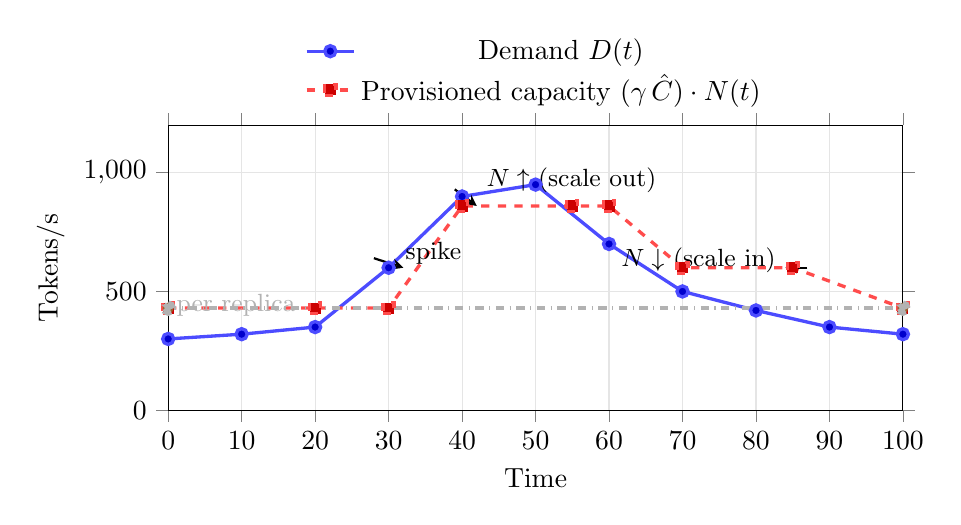
\begin{tikzpicture}
\begin{axis}[
    width=0.9\linewidth,
    height=5.2cm,
    xlabel={Time},
    ylabel={Tokens/s},
    ymin=0, ymax=1200,
    xmin=0, xmax=100,
    grid=both, grid style={gray!20},
    legend style={at={(0.5,1.03)},anchor=south,draw=none,fill=none},
    tick align=outside
]
% Demand (tokens/s)
\addplot+[very thick, blue!70] coordinates {
(0,300) (10,320) (20,350) (30,600) (40,900) (50,950) (60,700) (70,500) (80,420) (90,350) (100,320)
};
\addlegendentry{Demand $D(t)$}

% Capacity with headroom gamma=0.7 (N changes)
\addplot+[very thick, dashed, red!70] coordinates {
(0,430) (20,430) (30,430) (40,860) (55,860) (60,860) (70,600) (85,600) (100,430)
};
\addlegendentry{Provisioned capacity $(\gamma\,\hat{C})\cdot N(t)$}

% Horizontal line for single-replica capacity at gamma*C_hat
\addplot+[domain=0:100, samples=2, gray!60, dashdotted, ultra thick] {430};
\node[gray!60] at (axis cs:6,455) {\small $\gamma\,\hat{C}$ per replica};

% Annotations
\node[anchor=west] at (axis cs:31,660) {\small spike};
\draw[->,>=stealth,thick] (axis cs:28,640) -- (axis cs:32,600);

\node[anchor=west] at (axis cs:42,970) {\small $N\uparrow$ (scale out)};
\draw[->,>=stealth,thick] (axis cs:39,930) -- (axis cs:42,860);

\node[anchor=east] at (axis cs:84,630) {\small $N\downarrow$ (scale in)};
\draw[->,>=stealth,thick] (axis cs:87,600) -- (axis cs:84,600);

\end{axis}
\end{tikzpicture}
\end{llmfigbox}
\caption{Metrics-based target tracking. The autoscaler tracks demand $D(t)$, maintaining capacity above $D(t)$ using headroom $\gamma$ by adjusting replicas $N(t)$.}
\label{fig:autoscale-target-tracking}
\end{figure}

Figure~\ref{fig:autoscale-event-based} shows an event-driven autoscaling workflow that uses external triggers to pre-warm capacity ahead of traffic spikes.

\begin{figure}[htbp]
\centering
\begin{llmfigbox}
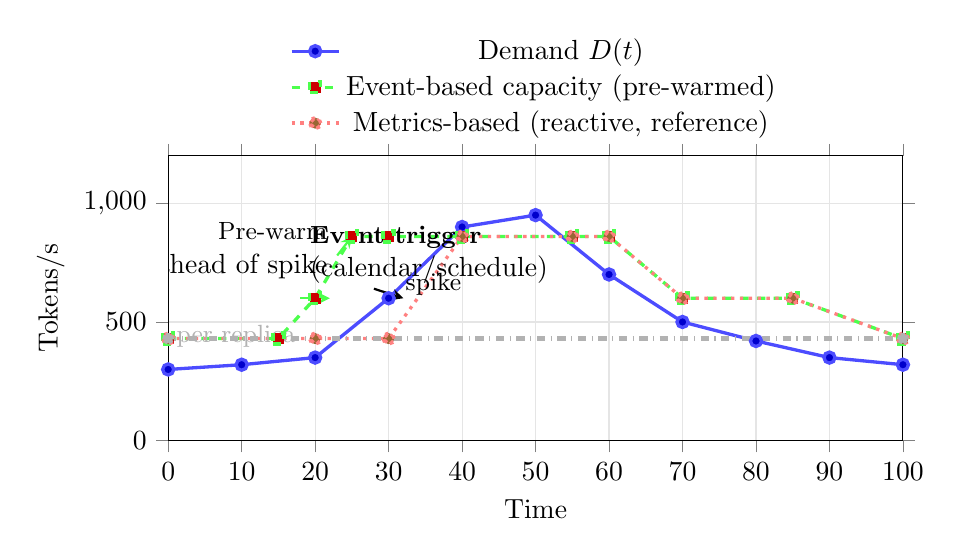
\begin{tikzpicture}
\begin{axis}[
    width=0.9\linewidth,
    height=5.2cm,
    xlabel={Time},
    ylabel={Tokens/s},
    ymin=0, ymax=1200,
    xmin=0, xmax=100,
    grid=both, grid style={gray!20},
    legend style={at={(0.5,1.03)},anchor=south,draw=none,fill=none},
    tick align=outside
]
% Demand (tokens/s) - same spike pattern
\addplot+[very thick, blue!70] coordinates {
(0,300) (10,320) (20,350) (30,600) (40,900) (50,950) (60,700) (70,500) (80,420) (90,350) (100,320)
};
\addlegendentry{Demand $D(t)$}

% Event-based capacity: pre-warms BEFORE spike (proactive)
\addplot+[very thick, dashed, green!70] coordinates {
(0,430) (15,430) (20,600) (25,860) (30,860) (40,860) (55,860) (60,860) (70,600) (85,600) (100,430)
};
\addlegendentry{Event-based capacity (pre-warmed)}

% Metrics-based capacity (reactive, shown for comparison)
\addplot+[very thick, dotted, red!50] coordinates {
(0,430) (20,430) (30,430) (40,860) (55,860) (60,860) (70,600) (85,600) (100,430)
};
\addlegendentry{Metrics-based (reactive, reference)}

% Horizontal line for single-replica capacity
\addplot+[domain=0:100, samples=2, gray!60, dashdotted, ultra thick] {430};
\node[gray!60] at (axis cs:6,455) {\small $\gamma\,\hat{C}$ per replica};

% Event trigger annotation
\node[anchor=south west, align=left] at (axis cs:18,620) {\small \textbf{Event trigger}\\(calendar/schedule)};
\draw[->,>=stealth,thick, green!70] (axis cs:18,600) -- (axis cs:22,600);

% Pre-warm annotation
\node[anchor=east, align=right] at (axis cs:23,800) {\small Pre-warm\\ahead of spike};
\draw[->,>=stealth,thick, green!70] (axis cs:23,780) -- (axis cs:25,860);

% Spike annotation
\node[anchor=west] at (axis cs:31,660) {\small spike};
\draw[->,>=stealth,thick] (axis cs:28,640) -- (axis cs:32,600);

\end{axis}
\end{tikzpicture}
\end{llmfigbox}
\caption{Event-based autoscaling with predictive pre-warming. Unlike reactive metrics-based scaling (dotted reference line), event-based scaling provisions capacity \emph{before} demand spikes arrive, leveraging calendar events or scheduled triggers. This eliminates cold-start latency and ensures capacity is ready when needed.}
\label{fig:autoscale-event-based}
\end{figure}

% ------------------------------------------------------------

\section{Caching for Scale}
\label{sec:caching}
Caching avoids recomputation for repeated work, reducing both latency and GPU load. In LLM systems, we consider two main types: response caching (caching model outputs for identical queries) and embedding caching (caching vector embeddings for identical pieces of text, to accelerate retrieval-augmented generation, \textsc{RAG}). Effective caching can significantly improve scalability by serving a portion of requests from memory instead of using scarce GPU cycles.

\subsection{Response Caching}
\label{sec:scaling-response-caching}
Response caching stores recent queries and their generated outputs, bypassing the model for exact matches. This is analogous to web caching for static content, but with additional considerations given the stochastic nature of LLM decoding.

\subsubsection{Key considerations}
\begin{itemize}
    \item \textbf{Cache key:} Must uniquely represent the query, model version, decoding parameters, and prompt template. Even minor changes in parameters (e.g., temperature, top-$p$) can alter outputs.
    \item \textbf{TTL (time-to-live):} Balance freshness with hit rate; short TTL for time-sensitive domains, longer for static domains (e.g., FAQ bots).
    \item \textbf{Storage backend:} Redis, Memcached, or in-process caches for low-latency access.
    \item \textbf{Invalidation:} Invalidate cache entries when upstream knowledge base changes.
\end{itemize}

\subsubsection{Optimizations}
\begin{itemize}
    \item \textbf{Partial match caching:} Store and reuse intermediate outputs (e.g., retrieval results) for partially overlapping queries.
    \item \textbf{Compression:} Apply lightweight compression (e.g., LZ4) to reduce memory footprint.
    \item \textbf{Popularity-based eviction:} Keep high-frequency queries pinned; use LFU eviction policy.
\end{itemize}

\subsubsection{Notes and context}
Beyond exact matches, caches can support partial reuse. For instance, if two queries share a long prefix, the work done for the first query’s response might be partially reused for the second (cf.\ prefix caching). Some systems cache not only final outputs but intermediate results (retrieved documents, prompt embeddings), allowing the pipeline to skip repeated sub-steps on subsequent requests. Prediction caches have been used in prior ML serving systems for similar reasons (e.g., Clipper’s prediction cache) \cite{rise.cs.berkeley.edu}. In LLM deployments, the same ideas apply with larger payloads and generative variability.

\subsubsection{Case in \ishtar{}}
A Redis-based response cache with a 15-minute TTL yielded a 7--12\% GPU load reduction during steady traffic and $>\!30\%$ during breaking news with repeated queries (measured via GPU utilization metrics comparing cache-hit vs.\ cache-miss request paths).

\subsection{Embedding Caching}
\label{sec:scaling-embedding-caching}
Embedding caching stores vector embeddings for repeated documents, passages, or chunks in \textsc{RAG} pipelines. In RAG systems, every unique document (or query) is transformed into an embedding by an encoder model; if the same document or query reappears, caching its embedding avoids redundant encoder forward passes.

\subsubsection{Key considerations}
\begin{itemize}
    \item \textbf{Cache key:} Deterministic hash of the document content plus embedding model identifier/version.
    \item \textbf{Persistence:} Use durable storage (e.g., Postgres with pgvector, FAISS on disk) to survive process restarts.
    \item \textbf{Invalidation:} Recompute and overwrite embeddings when content changes or model version updates.
\end{itemize}

\subsubsection{Optimizations}
\begin{itemize}
    \item \textbf{Lazy population:} Compute embeddings on first request; serve from cache thereafter.
    \item \textbf{Batch backfill:} For large document sets, precompute embeddings offline and populate the cache in bulk.
    \item \textbf{Sharding and replication:} Distribute embeddings across multiple storage nodes for scalability and redundancy.
    \item \textbf{Quantization:} Store compressed vector formats (e.g., FP16 or 8-bit) to reduce storage costs.
\end{itemize}

\subsubsection{Notes and context}
Persistence matters more for embedding caches: unlike response caches (which can often be purely in-memory), embedding caches benefit from durability so restarts do not cause mass re-embedding. Sharding and replication scale throughput and improve fault tolerance. At very large scales, storage pressure can be significant; product quantization or 8-bit storage reduces footprint at small accuracy cost, and many vector DBs (FAISS, Milvus) support compressed indexes out of the box.

\subsubsection{Case in \ishtar{}}
By hashing retrieved document chunks and caching embeddings in a pgvector-enabled Postgres cluster, \ishtar{} eliminated redundant embedding computation for $\sim$65\% of retrievals (measured via cache hit rate over a 7-day production window), cutting average RAG pipeline latency by 220\,ms (computed as the difference in end-to-end latency between cache-hit and cache-miss requests).

\medskip
\noindent\textbf{Summary.} Caching at both the response level and the embedding level contributed to the overall scalability of \ishtar{}. By avoiding recomputation, we effectively obtained more throughput from each GPU and served more users with the same hardware. The trade-off is additional complexity (key design, invalidation, persistence), but with careful engineering the benefits far outweigh the overhead.

Figure~\ref{fig:caching-flow} summarizes where common caching layers sit in the LLM request path and how they reduce repeated work.

\begin{figure}[htbp]
\centering
% ------------------------ (a) RESPONSE CACHE ------------------------
% \begin{subfigure}[b]{0.48\linewidth}
% \centering
% \begin{tikzpicture}[
%   node distance=6mm and 6mm,
%   box/.style={draw, rounded corners, thick, align=center, minimum width=2.8cm, minimum height=0.8cm, fill=gray!5},
%   store/.style={draw, rounded corners, thick, align=center, minimum width=2.8cm, minimum height=0.8cm, fill=blue!5},
%   io/.style={draw, rounded corners, thick, align=center, minimum width=2.2cm, minimum height=0.8cm, fill=green!5},
%   arr/.style={-{Stealth[length=2.5mm]}, thick}
% ]
% \node[io]   (client) {Client\\Request};
% \node[store, right=of client] (lookup) {Cache Lookup\\(Redis/Memcached)};
% \node[box, below=of lookup] (miss) {Miss};
% \node[box, right=of lookup, xshift=10mm] (hit) {Hit};
% \node[box, below=of miss] (infer) {LLM Inference\\(model + decode params)};
% \node[store, below=of infer] (store) {Store\\keyed by (query,\\model, params)};
% \node[io, right=of hit, xshift=10mm] (return1) {Return\\Cached Response};
% \node[io, below=of store] (return2) {Return\\New Response};

% % arrows
% \draw[arr] (client) -- (lookup);
% \draw[arr] (lookup) -- node[pos=0.5,left]{no} (miss);
% \draw[arr] (lookup) -- node[pos=0.5,above]{yes} (hit);
% \draw[arr] (miss) -- (infer);
% \draw[arr] (infer) -- (store);
% \draw[arr] (store) -- (return2);
% \draw[arr] (hit) -- (return1);
% \end{tikzpicture}
% \caption{Response cache: miss $\rightarrow$ infer $\rightarrow$ store $\rightarrow$ hit.}
% \end{subfigure}
% \hfill
% ------------------------ (b) EMBEDDING CACHE ------------------------
% \begin{subfigure}[b]{0.48\linewidth}
% \centering
% \begin{tikzpicture}[
%   node distance=6mm and 6mm,
%   box/.style={draw, rounded corners, thick, align=center, minimum width=2.8cm, minimum height=0.8cm, fill=gray!5},
%   store/.style={draw, rounded corners, thick, align=center, minimum width=2.8cm, minimum height=0.8cm, fill=orange!10},
%   io/.style={draw, rounded corners, thick, align=center, minimum width=2.4cm, minimum height=0.8cm, fill=green!5},
%   arr/.style={-{Stealth[length=2.5mm]}, thick}
% ]
% \node[io]   (text) {Text / Chunk};
% \node[box, right=of text] (hash) {Deterministic\\Hash\\(content + model)};
% \node[store, right=of hash] (elook) {Embedding Cache\\(pgvector/FAISS)};
% \node[box, below=of elook] (emiss) {Miss};
% \node[box, right=of elook, xshift=10mm] (ehit) {Hit};
% \node[box, below=of emiss] (encode) {Encoder\\(embed model)};
% \node[store, below=of encode] (estore) {Store\\(key $\to$ vector)};
% \node[io, right=of ehit, xshift=10mm] (usehit) {Use Vector\\(retriever/RAG)};
% \node[io, below=of estore] (usenew) {Use Vector\\(retriever/RAG)};

% % arrows
% \draw[arr] (text) -- (hash);
% \draw[arr] (hash) -- (elook);
% \draw[arr] (elook) -- node[pos=0.5,left]{no} (emiss);
% \draw[arr] (elook) -- node[pos=0.5,above]{yes} (ehit);
% \draw[arr] (emiss) -- (encode);
% \draw[arr] (encode) -- (estore);
% \draw[arr] (estore) -- (usenew);
% \draw[arr] (ehit) -- (usehit);
% \end{tikzpicture}
% \caption{Embedding cache: miss $\rightarrow$ encode $\rightarrow$ store $\rightarrow$ hit.}
% \end{subfigure}

\caption{Cache flow diagrams. \textbf{(a)} Response caching short-circuits identical requests; keys include query, model version, and decoding parameters. \textbf{(b)} Embedding caching avoids redundant encoder passes for repeated chunks; keys hash content + embedding model identity.}
\label{fig:caching-flow}
\end{figure}

\section{Cost-Aware Scaling}
\label{sec:cost-aware-scaling}
Beyond just technical performance, scaling strategies must account for cost efficiency. In practice, serving large models is expensive, so deploying them sustainably requires strategies to optimize the cost per query (or per token). Some guidelines and techniques for cost-aware scaling include:

\begin{itemize}
    \item Mix instance types for different workloads.
    \item Use spot/preemptible instances where possible.
    \item Route low-priority queries to smaller, cheaper models.
\end{itemize}
For \ishtar{}, critical fact-checking requests go to high-accuracy models, while background summarization uses smaller models.

\subsubsection{Mix instance types}
Use high-end GPUs only for latency-critical or very heavy workloads, and route lighter or non-urgent jobs to cheaper hardware (even if it is slower). For instance, one might use a few A100/H100 nodes for interactive queries, but send batch processing or long-running jobs to clusters of T4 or CPU instances overnight. This way, the expensive GPUs are utilized only for what truly needs them.

\subsubsection{Spot/preemptible capacity}
Many cloud providers offer spare capacity at much lower prices (e.g., AWS Spot, Azure Low-Priority VMs, GCP Preemptible VMs). The downside is they can be terminated with short notice. However, for elastic portions of your workload (background tasks or burst capacity), leveraging these can drastically cut costs. Systems like SpotServe have shown it is feasible to serve LLMs on spot instances by using fast checkpointing---saving model state at token boundaries so if an instance dies, work is not lost \cite{pope2023exegpt}. SpotServe introduces a mechanism to commit partial decoding progress so another instance can resume, achieving cost savings with minimal impact on users.

\subsubsection{Autoscale down aggressively}
Idle GPUs burn money. Ensure your autoscaling (Section~\ref{sec:autoscaling}) scales in when load drops. It can even be worth it to shut down to zero during off-hours (if the model can be re-loaded relatively quickly when needed). Also consider using GPU time-sharing (if supported)---e.g., run two small models on one GPU when volumes are low, instead of each on separate GPUs, to increase utilization.

\subsubsection{Batching for cost}
Optimize batch size for cost, not just latency: running at maximum throughput (full GPU utilization) yields the lowest cost per token, but might introduce latency. Decide on an acceptable latency target and within that, push batch sizes as high as possible. Many deployments find a sweet spot where slight latency sacrifice (e.g., 50\,ms slower) can double throughput, thus halving cost per query. It is a business decision how much latency one can trade for cost savings.

\subsubsection{Multi-model serving and routing}
Often, one can deploy a family of models of different sizes and costs, and route queries intelligently. For example, some requests can be satisfied by a 7B or 13B model, while only a subset truly require a 70B model. A router (possibly a small classifier) predicts which model is sufficient for a given query. By doing so, average cost per query can be brought down significantly, since only a fraction of queries hit the largest model.

\subsubsection{Throughput-oriented R\&D}
Optimize your deployment as if you were optimizing a training job---profile bottlenecks, try quantization, faster kernels, etc. Every 10\% speedup is 10\% cost reduction if you can do the same work with fewer GPU-seconds. Techniques covered in Chapter~\ref{ch:performance} (quantization, pruning, better kernels) directly translate to cost savings when deployed at scale.

\subsubsection{Case in \ishtar{}}
In \ishtar{}, we implemented a multi-tier model approach as mentioned: critical fact-checking or editing requests went to a high-accuracy, large model, whereas routine summarizations or drafts used a smaller distilled model. This yielded large cost reductions by serving a portion of queries on cheap infrastructure. We also aggressively used spot instances for non-critical scaling---at one point, 50\% of our GPUs were spot (based on fleet composition during a cost-optimization period), saving an estimated 40\% in GPU-hours (calculated from spot vs.\ on-demand pricing differentials and actual usage), and the system seamlessly failed over to on-demand when a spot instance occasionally evicted (thanks to fast checkpointing of the KV cache).

\subsubsection{Automated cost planners}
Another research prototype called Melange takes cost-awareness further by automatically selecting the cheapest combination of heterogeneous instances to meet an LLM service's SLOs \cite{pope2023exegpt}. It considers the request rate, size, and latency target, then navigates cloud instance options (GPU types, counts, prices) to find an optimal deployment plan \cite{pope2023exegpt}. Such systems hint at a future where, given a budget constraint, the infrastructure could dynamically reconfigure to minimize cost (even moving across regions for price arbitrage, if latency allows).

\medskip
\noindent\textbf{Summary.} Scaling up LLM deployments is not just about raw performance---it is about doing so economically. Cost-aware scaling techniques ensure that as we serve more users and more queries, the cloud bill scales sub-linearly or stays within budget. This often entails embracing complexity (hybrid models, spot markets, etc.) for significant savings.

\section{Scaling Retrieval-Augmented Generation (RAG)}
\label{sec:scaling-rag}
Many LLM applications augment the base model with a retrieval step---fetching relevant documents from a knowledge base to ground the model’s responses. Scaling RAG introduces its own challenges, as both the retrieval system and the generator must scale in tandem. As knowledge bases grow, retrieval can become a bottleneck:
\begin{itemize}
    \item Shard indexes across multiple vector DB nodes.
    \item Use approximate nearest neighbor search for speed.
    \item Keep hot data in memory for low-latency retrieval.
\end{itemize}

\subsubsection{Index sharding}
As the corpus grows (potentially to millions of documents or more), a single vector index may not handle the load or may not fit in memory. Sharding the index across multiple servers (or using a distributed vector database) allows parallel searches. For example, splitting an index into $k$ shards and querying them in parallel can nearly maintain per-query latency even as data scales $k\times$. This is essentially horizontal scaling for the retriever.

\subsubsection{Approximate nearest neighbor (ANN) search}
Using algorithms like HNSW, IVF, or product quantization can dramatically speed up retrieval with minimal loss in relevance. At large scale, exact nearest neighbor search in high dimensions is often infeasible. ANN methods allow sub-linear time queries and much smaller memory footprints, trading a tiny bit of accuracy for huge speed gains. This is crucial for real-time RAG.

\subsubsection{Hot tiers and in-memory caches}
For corpora that are partially hot (frequently queried documents) and cold (rarely queried), it makes sense to keep the hot subset in GPU or RAM for fast access, and store the rest on slower storage. In practice, this might mean maintaining an in-memory cache of popular vectors, or using a two-tier index (first check a smaller high-speed index of popular items, then the full index if needed). This ensures low latency on the majority of queries that hit popular content.

\subsubsection{Overlap retrieval with generation}
RAG is often implemented sequentially (retrieve then generate). When the model is large and slow, consider overlapping retrieval and generation for different segments of the response. For instance, fetch the first chunk, start generation, and concurrently fetch the next chunk(s) while the model writes the beginning of the answer. Coordination is non-trivial, but overlapping can hide retrieval latency behind ongoing decoding.

\subsubsection{Recent directions}
Sparse RAG (2023) observed that one major cost in RAG is that retrieved documents lengthen the model’s input, causing more attention computation \cite{pope2023exegpt}. It proposed encoding retrieved docs in parallel (outside the main model) to avoid the quadratic attention cost, and then using control tokens to let the model selectively attend only to the most relevant information \cite{pope2023exegpt}. Another work, RAGCache, targets redundancy across queries \cite{pope2023exegpt}: it caches intermediate states of the external knowledge (e.g., a ``knowledge tree’’ of frequently co-retrieved items) so multiple queries can reuse shared representations rather than recomputing from scratch \cite{pope2023exegpt}. These approaches reduce both retrieval latency and the amount of text fed repeatedly into the model.

\subsubsection{Case in \ishtar{}}
Scaling RAG in \ishtar{} meant scaling the vector search backend alongside the model. We sharded a FAISS index of news articles into three shards (one per region data center) and used locality-aware querying (users in Europe query the EU shard first, etc.) to minimize latency. We also pre-computed and cached embeddings for the top 100k most-read articles. This way, when those articles were retrieved as context, we already had their vectors and could also skip re-embedding them for generation (as described in Section~\ref{sec:scaling-event-autoscaling}). Through these measures, we maintained end-to-end RAG query latencies under 1\,s even as our knowledge base grew by tens of thousands of articles per day.

\medskip
\noindent\textbf{Summary.} Scaling RAG is a multidimensional challenge: IR-side scaling (index sharding, ANN, hot tiers, caching) must go hand-in-hand with LLM-side scaling (batching, KV management, and context-efficient prompting). Marrying these efficiently is an active area of systems research.

Figure~\ref{fig:rag-two-tier} sketches a practical two-tier RAG serving layout that separates hot and cold data while keeping latency predictable.

\begin{figure}[htbp]
\centering
\begin{llmfigbox}
\begin{tikzpicture}[
  node distance=7mm and 9mm,
  box/.style={draw, rounded corners, thick, align=center, minimum width=2.9cm, minimum height=0.9cm, fill=gray!5},
  hot/.style={draw, rounded corners, thick, align=center, minimum width=3.2cm, minimum height=0.9cm, fill=orange!12},
  dist/.style={draw, rounded corners, thick, align=center, minimum width=3.2cm, minimum height=0.9cm, fill=blue!7},
  stor/.style={draw, rounded corners, thick, align=center, minimum width=3.2cm, minimum height=0.9cm, fill=green!10},
  arr/.style={-{Stealth[length=2.6mm]}, thick}
]

% Row 1: Query & Router
\node[box] (q) {User Query};
\node[box, right=of q] (route) {RAG Router\\(Query parse + features)};

% Row 2: Hot tier + cache
\node[hot, below=of route] (hotidx) {Hot Tier Index\\(in-memory / GPU)};
\node[stor, right=of hotidx, xshift=8mm] (embcache) {Precomputed Embedding Cache\\(hash(content) $\to$ vector)};

% Row 3: Sharded backend
\node[dist, below left=11mm and -2mm of hotidx] (sh1) {Shard 1};
\node[dist, below=11mm of hotidx] (sh2) {Shard 2};
\node[dist, below right=11mm and -2mm of hotidx] (sh3) {Shard 3};

% Row 4: Merge + rank + generator
\node[box, below=15mm of sh2] (merge) {Merge \& (Re)Rank\\(ANN results aggregate)};
\node[box, right=20mm of merge] (gen) {Generator (LLM)\\(assemble context + decode)};

% Edges: query path
\draw[arr] (q) -- (route);

% Hot tier lookup
\draw[arr] (route) -- node[pos=0.5,right,sloped]{first lookup} (hotidx);

% Hit path from hot to merge
\draw[arr] (hotidx) -- node[pos=0.5,left]{hit} (merge);

% Miss path to shards
\draw[arr] (hotidx.west) .. controls +(-2.0,0.0) and +(0.0,1.2) .. node[pos=0.29,above]{miss} (sh1.north);
\draw[arr] (hotidx) -- (sh2.north);
\draw[arr] (hotidx.east) .. controls +(2.0,0.0) and +(0.0,1.2) .. (sh3.north);

% Shards back to merge
\draw[arr] (sh1) -- (merge);
\draw[arr] (sh2) -- (merge);
\draw[arr] (sh3) -- (merge);

% Embedding cache notes/edges
\node[align=left, font=\small] (note) at ($(embcache.north)+(0,1.0)$) {reuse vectors on\\ identical chunks};
\draw[-{Stealth[length=2.0mm]}, thick] (note.south) -- (embcache.north);

% Merge to generator
\draw[arr] (merge) -- (gen);

% Legend box (compact)
\node[draw, rounded corners, thick, align=left, anchor=north west, fill=white, inner sep=2mm] at ($(q.north west)+(-1.0,1.0)$) (leg) {%
\textbf{Two-tier RAG}\\[1pt]
\textbf{Hot tier:} recent/popular items in RAM/GPU\\
\textbf{Fallback:} parallel ANN on sharded index\\
\textbf{Cache:} precomputed embeddings (hash$\to$vec)\\
\textbf{Output:} merged top-$k$ to LLM
};

\end{tikzpicture}
\end{llmfigbox}
\caption{Two-tier RAG scaling. A router first probes a \emph{hot} in-memory/GPU tier; on miss, it falls back to a \emph{distributed} (sharded) ANN index in parallel. Precomputed embedding cache avoids redundant encoding. Results are merged/re-ranked, then fed to the generator.}
\label{fig:rag-two-tier}
\end{figure}

\section{Geographic Scaling}
\label{sec:geo-scaling}
Geographic scaling refers to deploying LLM services across multiple distant regions or data centers to serve users around the globe with low latency and to meet data residency requirements. In essence, it is horizontal scaling across geography.

Deploy regional inference clusters to:
\begin{itemize}
    \item Reduce latency for local users.
    \item Comply with data residency laws.
\end{itemize}
\ishtar{} maintains clusters in North America, Europe, and Asia.

\subsubsection{Latency and compliance benefits}
Deploying regional inference clusters can achieve: (a) latency reduction---users connect to the nearest server, avoiding transcontinental network delays (often saving 50--150\,ms RTT for interactive workloads), and (b) regulatory compliance---certain jurisdictions require that user data (and by extension, model processing of that data) remain in-region (e.g., EU data in the EU).

\subsubsection{Model placement strategies}
\emph{Replicate vs.\ partition.} The simplest approach is to replicate the entire model and pipeline in each region (low latency, higher cost). Alternatives include hub-and-spoke layouts (central region hosts the largest model; edges host smaller models, caches, or pre/post-processing). Replication ensures consistent latency for all users; partial replication reduces GPU footprint at the cost of some cross-region hops.

\subsubsection{Consistency, versioning, and caches}
If multiple regions host models, keep them aligned on weights, prompts, and policy. Users moving between regions should see consistent behavior, implying global deployment orchestration. Caches are usually per-region (for performance and simplicity), so duplicates across regions are acceptable; cross-region cache sharing is rarely worthwhile due to latency.

\subsubsection{Traffic routing and failover}
Use geo-aware DNS or global traffic managers to route users to the nearest or healthiest region. For failover, overflow or outage traffic can be routed to a secondary region (with a latency penalty). Anycast and cloud traffic managers help maintain high availability with policy-based routing.

\subsubsection{Data compliance controls}
Ensure sensitive data does not cross regions: enforce geo-fencing at the application and networking layers. If a user from region~$X$ hits region~$Y$, forward or deny based on compliance posture.

\subsubsection{Edge acceleration vs.\ full serving}
Some deployments use smaller ``edge'' models or caches: edge sites handle easy queries locally and forward only complex ones to a central model. Hybrid setups can run speech-to-text or retrieval locally and send compact representations to the central LLM, trading compute for latency.

\subsubsection{Decentralized precedent (Petals)}
Petals demonstrated geo-distributed inference over a volunteer network of GPU nodes hosting shards of very large models (e.g., BLOOM-176B), achieving interactive speeds by pooling global resources \cite{pope2023exegpt,helix2023}. While the volunteer setting is unique, similar ideas appear in enterprise multi-region pools (with stronger SLAs): aggregate GPU capacity across regions and rebalance as load shifts. Petals addressed unpredictable latencies and node churn with fault-tolerant protocols and dynamic rebalancing \cite{pope2023exegpt}.

\subsubsection{Industrial practice}
In production, most organizations replicate models regionally for reliability and latency. For example, multiple Azure regions host ChatGPT for proximity to users. Similarly, \ishtar{} maintained clusters in North America, Europe, and Asia, each capable of serving local traffic independently; if one region went down or saturated, traffic shifted to another region with a controlled performance penalty.

\subsubsection{Networking and future directions}
Private backbones and smart routing let providers forward requests to a near-optimal region (not always the physically closest) under load. CDN-like strategies for LLMs may emerge, caching not static assets but popular ``prompt--response'' pairs or compact intermediate representations.

\medskip
\noindent\textbf{Summary.} Geographic scaling reduces user-perceived latency and meets local policies at the cost of added operational complexity. It is the outermost layer of scale: after optimizing single- and multi-node serving, the final frontier is scaling across continents.

Figure~\ref{fig:geo-scaling-inset} depicts a typical multi-region serving topology with geo-routing, regional caches, and failover paths.

\begin{figure}[htbp]
\centering
\begin{llmfigbox}
\begin{tikzpicture}[
  node distance=6mm and 12mm,
  region/.style={draw, rounded corners, thick, minimum width=2.9cm, minimum height=1.0cm, align=center, fill=gray!5},
  user/.style={draw, rounded corners, thick, minimum width=2.2cm, minimum height=0.8cm, align=center, fill=green!8},
  arr/.style={-{Stealth[length=2.6mm]}, thick},
  fail/.style={-{Stealth[length=2.6mm]}, thick, dashed, color=red!70}
]
% Schematic world frame (purely illustrative)
\node[draw, rounded corners, thick, minimum width=11.5cm, minimum height=5.2cm, fill=blue!2] (frame) {};

% Regions (left-to-right placement)
\node[region, anchor=west] (na) at ($(frame.west)+(0.6,0)$) {North America\\(NA cluster)};
\node[region] (eu) at ($(frame.center)+(0,1.0)$) {Europe\\(EU cluster)};
\node[region, anchor=east] (ap) at ($(frame.east)+(-0.6,0)$) {Asia-Pacific\\(APAC cluster)};

% Users (example clients)
\node[user, above=of na] (userna) {Users (NA)};
\node[user, above=of eu] (usereu) {Users (EU)};
\node[user, above=of ap] (userap) {Users (APAC)};

% Primary routing (nearest region)
\draw[arr] (userna) -- node[pos=0.5,right]{nearest} (na.north);
\draw[arr] (usereu) -- node[pos=0.5,right]{nearest} (eu.north);
\draw[arr] (userap) -- node[pos=0.5,right]{nearest} (ap.north);

% Failover paths (between regional clusters)
\draw[fail] (na.east) .. controls +(1.2,0.4) and +(-1.2,0.4) .. (eu.west) node[pos=0.52,above,sloped] {\small failover};
\draw[fail] (eu.east) .. controls +(1.2,-0.4) and +(-1.2,-0.4) .. (ap.west) node[pos=0.52,below,sloped] {\small failover};
\draw[fail] (na.south east) .. controls +(1.4,-1.2) and +(-1.4,-1.2) .. (ap.south west) node[pos=0.5,below,sloped] {\small overflow};

% Compliance / geofencing note
\node[draw, rounded corners, align=left, anchor=south west, fill=white, inner sep=2mm]
at ($(frame.south west)+(0.35,0.35)$) {\small
\textbf{Notes}\\
-- Geo-aware routing (latency)\\
-- Regional data residency\\
-- Per-region caches \& failover
};

\end{tikzpicture}
\end{llmfigbox}
\caption{Geographic scaling schematic. Users are routed to the nearest regional cluster (NA/EU/APAC) for latency and data residency; dashed links illustrate failover/overflow between regions.}
\label{fig:geo-scaling-inset}
\end{figure}

\section{Case Study: Scaling Ishtar AI}
\label{sec:scaling-ishtar-case-study}
To ground the above concepts, we reflect on how \ishtar{}'s deployment evolved through several stages as demand grew. This progression illustrates the typical steps in scaling an LLM service from a small pilot to a global operation.

\subsection{Initial State}
\label{sec:scaling-ishtar-initial}
One GPU server with limited capacity, suitable for early trials.

In the earliest stage, \ishtar{} ran on a single GPU server with limited capacity. This was sufficient for early trials and internal demos. We used an off-the-shelf 13B parameter model, hosted on one NVIDIA A100 GPU with 40\,GB memory. There was no redundancy or autoscaling --- if the server went down, the service was offline (which was acceptable during prototyping). This setup handled only a few requests at a time with high latency (several seconds per query for longer articles). Batching was minimal and caching was not yet implemented. The focus at this stage was simply to validate the application’s functionality.

\subsection{Intermediate Stage}
\label{sec:scaling-ishtar-intermediate}
Multiple A100 servers behind a Kubernetes-based load balancer, dynamic batching enabled.

As usage grew, we moved to a cluster of multiple A100 GPU servers behind a Kubernetes-based load balancer. The model (now a fine-tuned 30B) was containerized, and we deployed 4 replicas to start, scaling up to 8 during peak hours. Horizontal scaling and basic autoscaling were introduced --- Kubernetes HPA (Horizontal Pod Autoscaler) based on GPU utilization. We enabled dynamic batching in the inference server, which significantly improved throughput (we observed up to 5--6$\times$ throughput increase when 8 requests were batched). At this stage, we also rolled out a simple response cache (in-memory within each pod) to cache exact question--answer pairs for a short time. This intermediate setup could handle moderate newsroom traffic, though it sometimes struggled with big spikes. Latency was brought down into the 1--2\,s range for most queries, thanks to batching and the move from CPU-bound parts (like some preprocessing) to GPU. We also started using monitoring dashboards to track p95 latency and utilization, feeding those into refined autoscaling rules.

\subsection{Mature Stage}
\label{sec:scaling-ishtar-mature}
Multi-region H100 clusters with automated scaling policies, caching layers, and tiered model serving.

In the mature stage, \ishtar{} became a multi-region, multi-tier deployment. We upgraded to clusters of H100 GPUs for core serving, as the model had grown to 70B with a 32k context. Each region (US-East, EU-West, APAC) had a cluster with auto-provisioning via Terraform and Kubernetes. We implemented the hybrid scaling strategy: a baseline of high-end GPUs always running for low latency, plus the ability to burst with additional GPUs (including spot instances) during events. Caching was now multi-layer: a Redis global response cache (shared by all pods in a region) and a distributed embedding cache using a vector DB for the document index. We had also introduced speculative decoding in this stage (running a 6B draft model alongside), which gave roughly a 1.5$\times$ speedup on long text generation. The system employed sophisticated autoscaling signals including predictive triggers for known events (as discussed in Section~\ref{sec:scaling-event-autoscaling}). Multi-tenancy was in effect: the platform served both our internal journalists and external API consumers, with priority scheduling ensuring the internal users (journalists) had reserved capacity during crunch time. By the time of this mature setup, \ishtar{} was sustaining peaks of $\sim$100 requests per second with median latency $<\!800$\,ms and p99 around 2\,s, across a user base spanning three continents. The scalability groundwork --- everything from model optimizations to geo-distributed clusters --- allowed it to handle major news surges (10$\times$ traffic in minutes) without failing. This final architecture reflects many best practices we have covered: mixed vertical/horizontal scaling, distributed inference techniques, aggressive batching, autoscaling, caching layers, and cost-awareness (spot instances, multi-model routing for efficiency).

Figure~\ref{fig:ishtar-timeline} summarizes the evolution of \ishtar{} from a single-GPU prototype to a multi-region, multi-tier production deployment.

\begin{figure}[htbp]
\centering
\begin{llmfigbox}
\begin{tikzpicture}[
  >=Stealth,
  milestone/.style={draw, rounded corners, thick, align=left, minimum width=4.8cm, minimum height=0.95cm, fill=gray!5, inner sep=3pt},
  label/.style={font=\small, align=left}
]

% Timeline axis
\draw[thick] (0,0) -- (15,0);

% Ticks
\foreach \x/\name in {0/Initial, 7/Intermediate, 14/Mature}
  \draw[thick] (\x,0.15) -- (\x,-0.15) node[below=2mm,font=\bfseries] {\name};

% Milestones (boxes)
\node[milestone, anchor=north west] (m0) at (-0.2,-1.8) {%
\textbf{Initial Stage}\\
-- Single GPU server (A100-40\,GB)\\
-- 13B off-the-shelf model\\
-- Minimal batching; no caching\\
-- High latency; prototype focus};

\node[milestone, anchor=north] (m1) at (7,-1.8) {%
\textbf{Intermediate Stage}\\
-- Multiple A100s; K8s load-balancer\\
-- 30B fine-tuned model; 4--8 replicas\\
-- Dynamic batching (5--6$\times$ gain)\\
-- Pod-local response cache; HPA};

\node[milestone, anchor=north east] (m2) at (15.2,-1.8) {%
\textbf{Mature Stage}\\
-- Multi-region H100 clusters (US/EU/APAC)\\
-- 70B model, 32k context; hybrid scaling\\
-- Redis response cache \& vector DB embeddings\\
-- Speculative decoding; predictive autoscaling};

% Connectors (from ticks to boxes)
\draw[->, thick] (0,-0.2) -- (m0.north west);
\draw[->, thick] (7,-0.2) -- (m1.north);
\draw[->, thick] (14,-0.2) -- (m2.north east);

% Legend
\node[draw, rounded corners, thick, align=left, fill=white, inner sep=2mm, anchor=north west]
at (-0.2,1.0) {\small
\textbf{Key milestones}\\
$\bullet$ Batching \& caching evolve with scale\\
$\bullet$ Autoscaling: reactive $\to$ predictive\\
$\bullet$ Tiered models \& spot for cost-awareness
};

\end{tikzpicture}
\end{llmfigbox}
\caption{\ishtar{} scaling timeline. The system evolved from a single-GPU prototype to a multi-region, multi-tier deployment with advanced batching, caching, speculative decoding, and predictive autoscaling.}
\label{fig:ishtar-timeline}
\end{figure}

\section{Best Practices Checklist}
\label{sec:scaling-best-practices}
In conclusion, scaling up LLM deployments involves a combination of strategic planning and tactical optimizations. The following checklist distills best practices:

\begin{tcolorbox}[
  title={\textbf{Best Practices Checklist for Scaling LLM Deployments}},
  colback=teal!5,
  colframe=teal!40!black,
  colbacktitle=teal!20,
  coltitle=black,
  fonttitle=\bfseries,
  boxrule=0.7pt,
  arc=4pt,
  left=3mm, right=3mm, top=3mm, bottom=3mm
]
\small
\setlength{\tabcolsep}{6pt}
\renewcommand{\arraystretch}{1.4}
\begin{tabularx}{\linewidth}{@{}p{3.2cm}X@{}}
\rowcolor{teal!15}
\textbf{Checklist Item} & \textbf{Description} \\
\midrule
\rowcolor{teal!8}
\textbf{Plan for Demand} & Start with capacity planning and demand forecasting to avoid constantly playing catch-up. Use historical data (or analogues) to predict peak loads, and design your system with some headroom. \\
\rowcolor{teal!3}
\textbf{Leverage Mixed Scaling} & Don't rely on just vertical or just horizontal scaling. Use a mix – vertical for performance, horizontal for flexibility. Many successful deployments use moderate per-node power plus the ability to add nodes dynamically. \\
\rowcolor{teal!8}
\textbf{Optimize Inference Before Adding Hardware} & It's often cheaper to optimize software (batching, caching, quantization) than to throw more GPUs at the problem. Squeeze as much throughput as possible out of each GPU; measure cost per token as a key metric. \\
\rowcolor{teal!3}
\textbf{Implement Robust Autoscaling} & Automated scaling is essential for cost-effective operation. Use metrics to scale reactively and incorporate predictive or scheduled scaling for known patterns. Ensure you have safeguards (cooldowns, max/min bounds) to prevent thrashing. \\
\rowcolor{teal!8}
\textbf{Monitor and Iterate} & Continuously monitor latency percentiles, throughput, and utilization. These metrics will tell you where the bottlenecks are (e.g. if GPUs are underutilized, maybe your batcher is too conservative; if latency spikes, maybe a particular component is slow or thrashing). \\
\rowcolor{teal!3}
\textbf{Use Caching Liberally} & Caching can drastically cut redundant work. Identify opportunities at all levels – from full response caching for repeated queries, to prefix caching within the model, to embedding caching in RAG. Even a small cache with a few GB of RAM can often handle a large fraction of repeat requests. \\
\rowcolor{teal!8}
\textbf{Geo-Distribute if User Base is Global} & The speed of light is a factor – serving from a single region will incur unavoidable latency for distant users. Plan a geo-deployment if your user base is worldwide or if data locality laws require it. This often comes after nailing down everything in one region first. \\
\rowcolor{teal!3}
\textbf{Gradual Rollout and Testing} & Scale incrementally. Test new scaling techniques (like speculative decoding or new batching algorithms) under load in a staging environment if possible. Each addition (e.g. a new cache layer, new parallelism) adds complexity; ensure it behaves as expected with your workload before relying on it in prod. \\
\end{tabularx}
\end{tcolorbox}

Scaling LLM systems requires balancing performance, cost, and complexity. By designing for scalability from the outset and drawing on the patterns discussed (from distributed inference to caching and autoscaling), teams can adapt rapidly to changing demands without sacrificing quality or breaking the bank. The story of \ishtar{} demonstrates that with careful planning and incorporation of cutting-edge techniques from academia and industry, even a resource-intensive LLM application can be made to operate reliably at scale. 

\medskip
\noindent\textbf{Scaling vs.\ Performance Optimization.} It is important to distinguish scaling (adding capacity to handle more load) from performance optimization (improving efficiency per unit of capacity). While this chapter has focused on scaling mechanisms---adding replicas, distributing inference, and provisioning capacity---these strategies must still respect fundamental performance constraints: Time-To-First-Token (TTFT), throughput per GPU, and cost per token. Simply scaling out without optimizing individual node performance can lead to inefficient deployments that consume excessive resources. In Chapter~\ref{ch:performance}, we turn to performance optimization techniques---quantization, kernel optimization, model compression, and advanced inference strategies---that improve the efficiency of each GPU and reduce cost per query. The relationship is complementary: scaling provides capacity headroom, while performance optimization ensures that capacity is used efficiently. A well-scaled system that ignores performance optimization wastes resources; a highly optimized system that cannot scale fails under load. Together, scaling and performance optimization enable LLM deployments that are both efficient and elastic.

\printbibliography[
  heading=subbibliography,
  segment=\therefsegment,
  resetnumbers=true
]
\section*{Chapter Summary}
Scaling LLM deployments is a multi-objective optimization problem across latency, throughput, reliability, and cost. The most impactful performance levers are usually systems techniques implemented in the serving runtime (continuous batching, scheduling, and KV-cache management), combined with distributed inference strategies such as parallelism, quantization, and speculative decoding. Operationally, autoscaling, caching, and geo-routing turn these techniques into reliable behavior under bursty demand and shifting traffic patterns. The \ishtar{} case study illustrates how these controls interact in practice, emphasizing that robust scaling depends on both algorithmic techniques and disciplined operations. However, scaling alone is insufficient: performance optimization (covered in Chapter~\ref{ch:performance}) ensures that scaled capacity operates efficiently, respecting TTFT, throughput, and cost constraints.